\documentclass[12pt]{article}
%\documentclass{extarticle}
%\documentclass[ecta,nameyear, draft]{econsocart}
%% Packages:
\usepackage[utf8]{inputenc}
\usepackage[LGR, T1]{fontenc}
\usepackage{graphicx}
\usepackage{subcaption}
\usepackage{cancel}
\usepackage{float}
%\usepackage{enumitem}  
\usepackage[inline, shortlabels]{enumitem}
\usepackage[reqno]{amsmath} % leqno if want equation number to the left by default
\usepackage{amsthm}
\usepackage{mathtools}
\usepackage{amssymb}
\usepackage{amsfonts}
\usepackage{eurosym}
\usepackage{geometry}
\usepackage{dsfont}
%\usepackage[backend=bibtex, maxcitenames=2, natbib=true,style=authoryear]{biblatex}
\usepackage{setspace}
\usepackage{natbib}
\usepackage{sectsty} % section fontsize
\usepackage[colorlinks]{hyperref}
\hypersetup{citecolor=blue,linkcolor=blue, urlcolor=blue}
\usepackage{pgfplots}
\usepackage{tikz}
\usetikzlibrary{patterns}
\usetikzlibrary{datavisualization}
\usetikzlibrary{datavisualization.formats.functions}
\usetikzlibrary{positioning}
\usetikzlibrary{intersections, pgfplots.fillbetween}
\usepackage[flushleft]{threeparttable}
\usepackage[multiple]{footmisc} % just for multiple footnote separated with comma


%% Commands/Theorems:
\theoremstyle{plain} % https://en.wikibooks.org/wiki/LaTeX/Theorems
\newtheorem{theorem}{Theorem}%[section]
\newtheorem{assumption}{Assumption}
\newtheorem{subassumption}{Assumption}[assumption]
\renewcommand{\thesubassumption}{\theassumption\alph{subassumption}}
\newtheorem{subassumptionbis}{}[assumption]
\renewcommand{\thesubassumptionbis}{(\roman{subassumptionbis})}
\newtheorem*{normalization}{Normalization}
%\newtheorem{proposition}{Proposition}
\newtheorem{proposition}{Proposition}
\newenvironment{assumptionbis}[1]
  {\renewcommand{\theassumption}{$D$\ref{#1}}%
   \addtocounter{assumption}{-1}%
   \begin{assumption}}
  {\end{assumption}}
\newenvironment{normalizationbis}[1]
  {\renewcommand{\thenormalization}{$D$\ref{#1}}%
   \addtocounter{normalization}{-1}%
   \begin{normalization}}
  {\end{normalization}}

%\newtheorem{Lemma}[theorem]{Lemma}
\newtheorem{Lemma}{Lemma}
\newtheorem{acknowledgement}[theorem]{Acknowledgement}
\newtheorem{algorithm}[theorem]{Algorithm}
%\newtheorem{assumption}[theorem]{Assumption}
\newtheorem{axiom}[theorem]{Axiom}
\newtheorem{case}[theorem]{Case}
\newtheorem{claim}[theorem]{Claim}
\newtheorem{conclusion}[theorem]{Conclusion}
\newtheorem{conjecture}[theorem]{Conjecture}
\newtheorem{corollary}{Corollary}
\newtheorem{criterion}[theorem]{Criterion}
\newtheorem{definition}[theorem]{Definition}
\newtheorem{example}[theorem]{Example}
\newtheorem{exercise}[theorem]{Exercise}
\newtheorem{notation}[theorem]{Notation}
\newtheorem{problem}[theorem]{Problem}
%\newtheorem{proposition}[theorem]{Proposition}
\newtheorem{remark}[theorem]{Remark}
\newtheorem{solution}[theorem]{Solution}
\newtheorem{summary}[theorem]{Summary}
\newtheorem{condition}{Condition}

%\newenvironment{proof}[1][Proof]{\noindent\textbf{#1.} }{\ \rule{0.5em}{0.5em}}

\newcommand*{\myfont}{\fontfamily{qpl}\selectfont}
\DeclareTextFontCommand{\textmyfont}{\myfont}

\renewcommand{\j}{\ensuremath{\text{j}}}
\newcommand{\qedblack}{\tag*{$\blacksquare$}}


\makeatletter
\newcommand{\leqnomode}{\tagsleft@true}
\newcommand{\reqnomode}{\tagsleft@false}
\makeatother


% Definitions
\def\mydoubleq#1{``#1''}
\def\mysingleq#1{`#1'}

% Notation for epsilon, Epsilon, eta, Eta
\DeclareSymbolFont{upgreek}{LGR}{cmr}{m}{n}
\SetSymbolFont{upgreek}{bold}{LGR}{cmr}{bx}{n}
%\DeclareMathSymbol{\Epsilon}{\mathord}{upgreek}{`E}
%\DeclareMathSymbol{\Eta}{\mathord}{upgreek}{`H}
% % and no need to specify eta and epsilon in this case. 
%

% https://tex.stackexchange.com/questions/183830/changing-math-fonts-for-greek-letters for the codes
\DeclareMathSymbol{\Epsilon}{\mathalpha}{letters}{"0F}
\DeclareMathSymbol{\Eta}{\mathalpha}{letters}{"11}
\DeclareMathSymbol{\epsilon}{\mathalpha}{letters}{`e}
\DeclareMathSymbol{\eta}{\mathalpha}{letters}{`h}



% Other:
\setcounter{MaxMatrixCols}{10}
\let\origtheassumption\theassumption


% Geometry of the document
%\geometry{left=.9in,right=.6in,top=1in,bottom=.9in}
\geometry{left=1.25in,right=1.25in,top=1.25in,bottom=1.25in}
%\sectionfont{\fontsize{16}{15}\selectfont}

\usepackage{changepage}
\newenvironment{widerequation}{%
    \begin{adjustwidth}{-2cm}{-2cm}\begin{equation}}
    {\end{equation}\end{adjustwidth}}
    



\usepackage{titlesec}
\titlespacing*{\section}{0pt}{19pt}{7pt}
\titlespacing*{\subsection}{0pt}{14pt}{5pt}
\titlespacing*{\subsubsection}{0pt}{12pt}{5pt}
\titlespacing*{\paragraph}{0pt}{9pt}{9pt}
\titleformat{\section}{\normalfont\fontsize{16}{15}\bfseries}{\thesection}{1em}{}
\titleformat{\subsection}{\normalfont\fontsize{14}{15}\bfseries}{\thesubsection}{1em}{}
\titleformat{\subsubsection}{\normalfont\fontsize{12}{15}\bfseries}{\thesubsubsection}{1em}{}

\allowdisplaybreaks





\begin{document}


%\newgeometry{top=1in} 

\title{{\fontsize{14}{20} \selectfont 
\vspace{-1cm}
\textbf{\textmyfont{Don't (fully) exclude me, it's not necessary! \\
Identification with semi-IVs}}}}

\author{{\fontsize{12}{20} Christophe Bruneel-Zupanc}\footnote{E-mail address: \href{mailto:christophe.bruneel@gmail.com}{christophe.bruneel@gmail.com}. I am especially grateful to Jad Beyhum, Geert Dhaene, and Alexandre Gaillard for their tremendous help, and to Gregory Veramendi for his help with the data. I also thank Laurens Cherchye, Edoardo Ciscato, Ben Deaner, Sebastian Fleitas, Ferre de Graeve, Olivier de Groote, Toru Kitagawa, Jan de Loecker, Iris Kesternich, Sebastiaan Maes, Thierry Magnac, Matt Masten, Arnaud Maurel, Costas Meghir, Erwin Ooghe, Christian Proebsting, Bram de Rock, Adam Rosen, Silvia Sarpietro, Jo Van Biesebroeck, Frank Verboven, Frederic Vermeulen, Ao Wang, Andrei Zeleneev, Mariana Zerpa, and participants to the seminars in Antwerp, Duke, Leuven, and Rotterdam for helpful discussions, suggestions, and comments. I acknowledge financial support from the Research Fund KU Leuven through the grant STG/21/040.} \\
{\fontsize{12}{20} Department of Economics, KU Leuven} } %\vspace{0.25cm}}
\date{{\fontsize{10}{20} \today}} 

%\vspace{-10cm}
\maketitle


\vspace{-0.20in}


\begin{abstract}
\renewcommand{\baselinestretch}{1.2} 
{\small

\noindent This paper proposes a novel tool to nonparametrically identify models with a discrete endogenous variable or treatment: \textit{semi-instrumental variables} (semi-IVs). 
A semi-IV is a variable that is relevant but only \textit{partially} excluded from the potential outcomes, i.e., excluded from at least one, but not necessarily all, potential outcome equations. 
It follows that standard instrumental variables (IVs), which are fully excluded from all the potential outcomes, are a special (extreme) case of semi-IVs. I show that full exclusion is stronger than necessary because the same objects that are usually identified with an IV \citep{angristimbens1994, heckmanvytlacil2005, chernozhukovhansen2005} can be identified with several semi-IVs instead, provided there is (at least) one semi-IV excluded from each potential outcome. 
For applied work, tackling endogeneity with semi-IVs instead of IVs should be an attractive alternative, since semi-IVs are easier to find: %semi-IVs are easier to find: 
most selection-specific costs or benefits can be valid semi-IVs, for example. The paper also provides a simple semi-IV GMM estimator for models with homogenous treatment effects and uses it to estimate the returns to education. \\

\noindent \textbf{Keywords:} exclusion restriction, instrumental variable, identification, nonseparable models, selection models, treatment effect.} \\ 
\end{abstract}



\restoregeometry
\setstretch{1.30} % check that gives 32 lines/page. Seems ok. 
\setlength{\abovedisplayskip}{6pt} % for skips before/after equations/align
\setlength{\belowdisplayskip}{6pt}





\pagebreak

\section{Introduction}

Since the seminal work of \cite{heckman1979}, endogenous selection is recognized as one of the main problems arising in empirical economics. A convenient strategy to deal with selection is to rely on instrumental variables (IVs), which are independent of the unobservables, relevant for the selection, and (fully) excluded from (all) the (potential) outcome equation(s) \citep[e.g.,][]{angrist1990, angristkrueger1991, angristimbens1994, card1995, angristimbensrubin1996, chernozhukovhansen2005}. In practice, however, instruments satisfying these conditions are hard to find. In particular, the exclusion restriction is especially difficult to satisfy and is often controversial, even for commonly used instruments. \\ 
\indent This paper provides a new approach to identify models with a discrete endogenous variable. %, relying on exclusions from the \textit{potential} outcomes, and not necessarily from `the' outcome. %\textcolor{red}{by applying exclusion restrictions to the potential outcomes, and not only to `the' outcome.} 
Instead of looking for an instrumental variable that is fully excluded from all the potential outcomes, one can look for several \textit{semi-instrumental variables} (semi-IVs) which are relevant for the selection, but only \textit{partially excluded} from the potential outcomes, i.e., excluded from at least one, but not necessarily all, potential outcome equations. %\\
\noindent For example, to identify the returns to college on earnings %at age $30$
\citep{angristkrueger1991, card1995, card2001, carneiroheckmanvytlacil2011}, one may use two semi-IVs: one that is excluded from the potential outcome of individuals if they go to college (college-goers) and one that is excluded from their potential outcome if they do not go (non-goers). 
The education-specific average local earnings/unemployment rate of other non-goers and goers, respectively, at the time of the decision (at age $17$) are good semi-IV candidates. 
First, both semi-IVs should be relevant for the selection: ceteris paribus, the better the current (at age $17$) local market conditions of educated individuals, the better the expectations of future earnings for college-goers, and the more likely one is to go. 
%First, both semi-IVs should be relevant for the selection: ceteris paribus, the better the current (at age $17$) local market conditions of educated individuals, the better the expectations about one's subsequent earnings if one decides to go to college, and the more likely one is to go. 
Because of serial correlation in local market conditions, the local conditions of older goers should correlate with, and not be excluded from the subsequent earnings (at age $30$) of individuals if they also decide to go to college (to be treated). 
On the contrary, apart from their effect on the selection, the local conditions of goers should be excluded from the subsequent earnings of individuals if they decide not to go, and do not receive any `treatment' (college education).  Conversely, the local conditions of non-goers are relevant for the selection, correlate with the subsequent earnings of non-goers, and should be excluded from the subsequent earnings of goers. 
Each semi-IV is only excluded from one of the two potential outcomes, but not from the other. Thus, these semi-IVs are not valid IVs. Importantly, the two semi-IVs are allowed to be correlated with one another. Hence the partial exclusion restriction means that, conditional on the non-excluded semi-IV, the other semi-IV is excluded. In general, selection-specific variables (e.g., costs and benefits associated with each alternative) naturally serve as semi-IVs, but valid semi-IVs are not limited to these. \\
%Attributes specific to a given alternative should be excluded from the outcome of individuals who picked another alternative. 
%\textcolor{red}{The (past) average local earnings of other college-goers, and non-goers at the time of the decision to go to college (at age $17$) are good semi-IV candidates. 
%The idea is that, at age $30$, the earnings of individuals who did not go to college are likely to depend on the past average local earnings of other non-goers, because of serial correlation in local labor market conditions, for example. However, controlling for this past average local earnings of non-goers, the past local earnings of college-goers should be excluded from the current earnings of non-goers, since the latter did not receive a college education. Vice versa, the past local earnings of non-goers should be excluded from the current earnings of goers. 
%The idea is that the subsequent earnings of non-goers are likely to depend on the current average local earnings of older non-goers, because of serial correlation in local labor market conditions, for example. However, controlling for the current local earnings of non-goers, the current earnings of goers should be excluded from the subsequent earnings of non-goers, since they will not have any college education.  Vice versa, the local earnings of non-goers should be excluded from the subsequent earnings of goers. %, but not from the earnings of non-goers. 
%Each semi-IV is only excluded from one of the two potential outcomes, but not from the other. As a consequence, these semi-IVs are not valid IVs in the usual sense.  
%Here, both semi-IVs should also be relevant for the selection into education: ceteris paribus, the better the expected local market conditions of college-goers, the more likely one is to go to college, and vice versa. 
%Importantly, the two semi-IVs are allowed to be correlated with each other. Hence the partial exclusion restriction means that, conditional on the non-excluded semi-IV, the other semi-IV is excluded. 
%In general, selection-specific variables (e.g., costs and benefits associated with each alternative) naturally serve as semi-IVs, but valid semi-IVs are not limited to these. \\ }
%
%
\indent I show that semi-IVs are sufficient to nonparametrically identify the same models and objects that are usually identified with IVs. In particular, quantile treatment effects (QTEs)  and individual treatment effects (ITEs) in nonseparable models with rank invariance imposed on the continuous potential outcomes \citep{chernozhukovhansen2005, vuongxu2017, bruneel2022}, as well as local average treatment effects (LATEs) and marginal treatment effects (MTEs) in generalized nonseparable selection (Roy) models with uniformity imposed on the selection equation \citep{angristimbens1994, heckmanvytlacil2005, heckmanvytlacil2007b}. 
The intuition is that, in models with discrete alternatives, a necessary condition for identification is, for each potential outcome, to have an exogenous source of variations that is excluded. However, contrary to what has been imposed so far in the literature on IVs, the excluded variation does not need to come from the same variable for each potential outcome. The full exclusion restriction is a theoretically convenient but very specific way to satisfy the identification condition and is, in fact, stronger than necessary. Indeed, it can also be more generally satisfied with several partially excluded semi-IVs instead. \\ %Identification can also be achieved with several partially excluded semi-IVs instead. \\
\indent The main cost of using semi-IVs instead of IVs, is the need to find multiple semi-IVs that jointly satisfy the necessary condition for identification. Moreover, semi-IVs need to satisfy stronger joint relevance conditions to identify the effects of the semi-IVs on the potential outcomes from which they are not excluded. 
However, in practice, the full exclusion restriction is often the main obstacle to finding a valid IV, and finding several relevant semi-IVs should be comparatively easier. Therefore, semi-IVs are a convenient alternative to address endogeneity in empirical work. \\ 
\indent For practical implementation, I also propose an easy-to-implement `semi-IV GMM' estimation procedure for additive models with homogenous treatment effects, in the spirit of standard IV GMM estimation \citep[as the Stata command, \texttt{ivreg},][]{baumetal2003}. I illustrate the method by estimating the returns to college using semi-IVs. \\
%
%
%
%

\noindent \textbf{Related literature} \\
\noindent There is a large literature on the identification of models with (nonseparable) endogeneity, and of treatment effects in such models \citep[e.g.,][]{angristimbens1994, angristimbensrubin1996, heckmanvytlacil1999, chesher2003, neweypowell2003, heckmanvytlacil2005, florensetal2008, imbensnewey2009}. %This paper builds a general approach that I study in the context of 
This paper studies nonparametric identification of two of the main general nonseparable models with discrete endogenous variables and heterogeneous treatment effects that are usually identified with IVs and span a large part of the literature: (i) the ‘IV-quantile regression' (IVQR) framework \citep{chernozhukovhansen2005, vuongxu2017, bruneel2022} and (ii) the LATE framework \citep{angristimbens1994}. 
These two frameworks are distinct and complementary. The IVQR setup places its main restrictions on the potential outcomes, requiring them to be continuous and monotone with respect to a common nonseparable unobserved variable (rank invariance). In its most advanced versions, it places almost no restrictions on the selection equation, and with a single relevant instrument, we can identify the entire model (and thus ITEs) with two \citep{vuongxu2017} or more \citep{bruneel2022} potential outcomes. 
The LATE framework does not restrict the (continuous or discrete) potential outcomes but imposes uniformity (also called monotonicity) on the effect of the instrument on the selection. This framework is equivalent to the generalized Roy model with nonseparable potential outcomes but separable unobservable heterogeneity in the latent index selection equation \citep{vytlacil2002, heckmanvytlacil2005, heckmanvytlacil2007b}. In this framework, we (only) identify some MTEs and LATEs, depending on the available instruments and the set of compliers they induce. 
I adapt both setups with semi-IVs and show that the same objects (ITEs, LATEs, MTEs, naturally adapted to the presence of semi-IVs) %, naturally redefined to account for the non-excluded semi-IVs) 
are still identified with semi-IVs as in the corresponding model with IVs. 
The main difference is that, without the full exclusion restriction, one needs to identify (and control for) the effect of the semi-IVs on the potential outcomes from which they are not excluded. This requires stronger relevance conditions on the effects of the semi-IVs on the selection. \\
%
%
%
\indent This paper also relates to numerous papers studying the identification of nonseparable models while relaxing some of the assumptions imposed on IVs \citep[see][for a recent review of the use of IVs in econometrics]{imbens2014}. For example, \cite{mogstadetal2021} obtain identification under a partial monotonicity condition. \cite{kitagawa2021} shows the identification power of various independence conditions imposed on the instruments. \cite{dhaultfoeuillefevrier2015}, \cite{torgovitsky2015}, and \cite{neweystouli2021} show identification of nonseparable models with continuous endogenous variables when the instruments have only limited support. Given the crucial role of IVs for identification, some papers also provide tests of instrument validity and/or exclusion restrictions \citep{kitagawa2015, caetanoetal2016, andresenhuber2021, dhaultfoeuilleetal2021}. 
Part of the literature shows that identification can sometimes be obtained without instruments, provided that certain specific conditions hold, e.g., conditional partial independence \citep{mastenpoirier2018}, identification at infinity \citep{dhaultfoeuilleetal2018}, identification based on heteroskedasticity \citep{kleinvella2010, lewbel2012, lewbel2018}, or local irrelevance of the instrument \citep{dhaultfoeuilleetal2021}. 
Finally, \cite{kolesaretal2013} show that identification can be obtained from many invalid instruments which may be correlated with the outcome (and thus not fully excluded) if the direct effects of these invalid instruments on the outcomes are uncorrelated with the effects of the instruments on the endogenous (continuous) regressor. In this case, one can use multiple invalid instruments to construct a valid instrument that can be used for identification. \\
%
\indent The identification approach in this paper differs from the aforementioned literature. I relax the full exclusion restriction imposed on IVs but not completely: the semi-IVs are still excluded from some (just not all) potential outcome equations. In contrast with the literature, I do not need to compensate for the relaxation of the exclusion restriction by adding structure to the model (e.g., specifying the distribution of the error terms or introducing other parametric assumptions). I let the semi-IVs enter the model in the most general nonparametric and nonseparable way, so identification does not come from parametric assumptions.  
The reason why I do not need to compensate for the relaxation of the full exclusion restriction is that, in fact, the full exclusion is stronger than necessary. Identification comes from having, for each potential outcome, an observable variable that yields exogenous variation and is excluded. Thus, identification can naturally be obtained with several partially excluded semi-IVs. 
Identification via targeted exclusion restrictions has been used in the original Roy model \citep{heckmanhonore1990} where the selection is restricted and uniquely determined by the direct comparison of the potential outcomes. However, in its extension with a general selection equation, i.e., in generalized and in extended Roy models \citep{heckmanvytlacil2007a, heckmanvytlacil2007b, abbringheckman2007, bayeretal2011, frenchtaber2011, dhaultfoeuillemaurel2013}, identification comes from standard arguments, using IVs or identification at infinity. In the case of a discrete endogenous choice (multiple unordered treatments), identification can be obtained with the exclusion of certain instruments from certain alternative-specific utilities driving the endogenous selection \citep{heckmanvytlacil2007b}. But in contrast with semi-IVs, these instruments are still fully excluded from the potential outcomes. 
To the best of my knowledge, thinking of exclusion restrictions in terms of potential outcomes instead of in terms of `the' outcome variable, and relying on partial exclusion from the potential outcomes for identification is new, especially in the context of general nonseparable models with heterogeneous treatment effects (both in the IVQR and LATE frameworks). 
This has important implications for empirical work because it allows researchers to look for semi-IVs in addition to fully excluded IVs to address endogeneity problems. \\ 
 \indent Section \ref{section_framework} considers nonparametric identification of models in the IVQR framework \citep{chernozhukovhansen2005, bruneel2022}. 
Section \ref{section_late} studies nonparametric identification of MTEs and LATEs in the LATE framework \citep{angristimbens1994, heckmanvytlacil2005}. 
Section \ref{section_ate} gives a closed-form expression for the average treatment effect in a simplified model with a homogenous treatment effect, as well as the corresponding semi-IV GMM estimator. I use it to estimate the returns to schooling with semi-IVs as an illustration. Section \ref{section_conclusion} concludes.  








\section{Nonseparable models with rank invariance}\label{section_framework}

In this section, I present the model and the principal identification results for the IVQR framework \citep{chernozhukovhansen2005}. First, to simplify the exposition of the constructive identification arguments, I focus on the case where the endogenous variable (treatment) is binary, $D=0$ or $D=1$, with one binary semi-IV for each potential outcome. However, the identification does not rely on these restrictions, and I provide the generalization with a discrete endogenous variable and general (not limited to binary, nor alternative-specific) semi-IVs in Section \ref{section_generalization}. % maybe add comment here for continuous semi-IVs? Let it in 2.2? 

\subsection{The Framework with binary endogenous choice}\label{subsection_framework_binary}
Consider the nonparametric, nonseparable, system of simultaneous equations %\\
\begin{align}\label{system_binary}
\left\{
    \begin{array}{l}
        Y_d = q_d(X, W_d, \Eta), \\
        D = b(X, W_0, W_1, \Eta, \Epsilon),  
    \end{array}
\right. \text{ for } d=0, 1.
\end{align}
Refer to the first line as the potential outcome equations and to the second line as the selection equation. $D \in \{0, 1\}$ is an observed (endogenous) binary choice/treatment, $Y_0$ and $Y_1$ are continuous potential outcomes. The researcher only observes a continuous outcome $Y$, which corresponds to the outcome in the selected alternative $D$, i.e., $Y = \sum^{1}_{d=0} Y_d \ \mathds{1}\{D=d\}.$ 
$X$ is a vector of observed exogenous covariates which affect the outcomes and the selection. 
A common nonseparable unobserved scalar shock, $\Eta$, is responsible for the heterogeneity of both potential outcomes at fixed $x$, and $w_d$. 
The nonseparable shock $\Eta$ can also affect the selection of the binary choice, yielding an endogeneity problem with respect to the outcome. 
In addition to $\Eta$, there exist other shocks, $\Epsilon$, which only affect the selection $D$. 
$W_0$ and $W_1$ are two binary semi-IVs that are relevant for the selection of the endogenous variable $D$, but are excluded from (at least) one of the two potential outcomes. 
$W_0$ (may) affect $Y_0$ but is excluded from $Y_1$ (controlling for $W_1$). Conversely, $W_1$ (may) affect $Y_1$ but is excluded from $Y_0$ (controlling for $W_0$). This is the main difference with the usual nonseparable triangular model with an instrumental variable, where the IV would enter the selection equation, but be fully excluded from the potential outcomes. \\
%
%
%
\indent The model also satisfies the following conditions. 
\begin{assumption}[Monotonicity]\label{ass_monot}
For each $d$, the potential outcomes functions are continuously differentiable and 
\begin{align*}
	\frac{\partial q_d(x, w_d, \eta)}{\partial \eta} > 0.
\end{align*}
\end{assumption}
\begin{normalization}\label{contshock} Conditional on $X=x$, $\Eta$ is continuously distributed as $\mathcal{U}(0,1)$.
\end{normalization}

\begin{assumption}[Independence]\label{indep_shock} Conditional on $X=x$, $(W_0, W_1)$ are independent from $\Eta$. 
\end{assumption}


\begin{assumption}[Support of the semi-IV]\label{supp_pev} For each $(w_0, w_1)$ in $\{0,1\}^2$, $\textrm{Pr}(W_0=w_0, W_1=w_1 |X) \neq 0$ almost surely for all $x$ in the support of $X$. \end{assumption}

\begin{assumption}[Regularity]\label{regularity} The selection function, $b(x, w_0, w_1, \Eta, \Epsilon)$, and the $\Epsilon$ shocks are such that $0 < \textrm{Pr}(D=d | X=x, W_0=w_0, W_1=w_1, \Eta=\eta) < 1$ for all $\eta, x$ and for each $(w_0, w_1) \in \{0,1\}^2$ and $d=0,1$. 
\end{assumption}





\indent Under Assumption \ref{ass_monot}, there is a one-to-one mapping between $\Eta$ and $Y_d$ for every $d, x, w_d$. This kind of monotonicity condition has been widely used for identification \citep{matzkin2003}, and it means that we only identify monotone effects of the unobserved nonseparable source of heterogeneity, $\Eta$ (which takes values $\eta$). A very important limitation of Assumption \ref{ass_monot} is that it requires a strictly continuous potential outcome for each alternative $d$. This rules out discrete response outcomes for example. 
Since the same $\Eta$ affects both potential outcomes in the model (\ref{system_binary}), the monotonicity implies \textit{rank invariance}. Indeed, the higher $\Eta$, the higher the relative rank in the distribution of $Y_0$ and $Y_1$. The rank invariance condition is slightly different from the standard rank invariance because here the semi-IVs also enter the potential outcome functions. 
Notice also that $\Eta$ is not directly identifiable from the data, so I normalize it to the uniform distribution, such that only the rank is identified. \\ 
\indent Assumption \ref{indep_shock} is a standard independence assumption between the semi-IVs and the unobserved variable. Importantly, $W_0$ and $W_1$ may be correlated with each other, as long as they are not perfectly correlated (which would violate Assumption \ref{supp_pev}). \\
\indent Assumption \ref{supp_pev} ensures that all the combinations of the semi-IVs occur in the data. Here it means that the support of $Z=(W_0, W_1)$ contains $2\times2=4$ different values which are all observed with non-zero probability for all $X=x$. \\
\indent I do not require independence between $\Epsilon$ and $\Eta$ or between $\Epsilon$ and $(W_0, W_1)$. The shock $\Epsilon$ is only present in the model to generate the selection probabilities, and I only require the regularity Assumption \ref{regularity} that we observe the full support of the potential outcomes $Y_d$ for each value of $(d, w_d, x)$. In fact, I could write the model without specifying the selection equation and $\Epsilon$ shocks. The only condition imposed on the selection is the regularity condition \ref{regularity}, i.e., that the selection probabilities are strictly greater than zero and below one for all $\Eta$.  \\ 
\indent This framework with binary treatment can be summarized by the `graph' in Figure \ref{fig_graph}. \\
%\indent Figure \ref{fig_graph} gives the `graph' summarizing this framework with binary treatment. \\ 


%\pagebreak 

\begin{figure}[h]
\centering
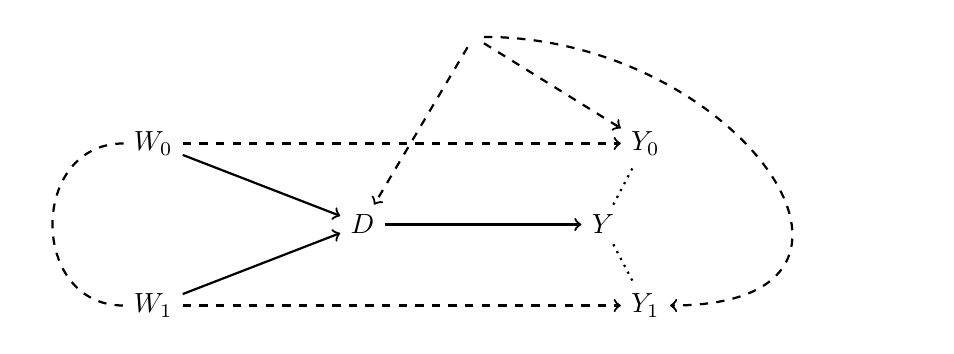
\begin{tikzpicture}[node distance={25mm}, thick] 
\node (D) {$D$}; 
\node (W0) [above left=0.5cm and 2cm of D]  {$W_0$}; 
\node (W1) [below left=0.5cm and 2cm of D]  {$W_1$}; 
\node (h) [above right=2cm and 1.cm of D] {$\Eta$}; 
\node (Y) [right=2.5cm of D]{$Y$}; 
\node (Y1) [below right=0.5cm and 3cm of D] {$Y_1$}; 
\node (Y0) [above right=0.5cm and 3cm of D] {$Y_0$}; 
\draw[->] (D) -- (Y); 
\draw[dotted] (Y) -- (Y1); 
\draw[dotted] (Y) -- (Y0); 
\draw[->] (W0) -- (D); 
\draw[->] (W1) -- (D);
\draw[dashed, ->] (W0) -- (Y0); 
\draw[dashed, ->] (W1) -- (Y1);
\draw[dashed] (W0) to [out=180,in=-180,looseness=1.5] (W1); 
\draw[dashed, ->] (h) -- (D); 
\draw[dashed, ->] (h) -- (Y0);
\draw[dashed, ->] (h) to [out=360,in=360,looseness=2] (Y1); 
\end{tikzpicture} 
\caption{Graph of the binary framework (without covariates $X$)}\label{fig_graph}
\end{figure}

\noindent \textbf{Example:} \\
%
%
%
\noindent Consider the standard example of the returns to education \citep{angristkrueger1991, card2001}. The binary endogenous decision is to go to college $(D=1)$ or not $(D=0)$. The potential outcomes are the earnings (at age $30$) of the individuals if they went to college ($Y_1$), or not ($Y_0$). $X$ represents demographics that influence both the choice to go (or not) and the outcomes. The nonseparable shock $\Eta$ represents individual unobserved ability. Ceteris paribus, a higher ability yields higher income, regardless of the chosen education, demographics, and local labor market conditions (rank invariance). $\Epsilon$ represents other unobserved factors influencing the decision to study or not, the preference for studying for example. 
%For the semi-IVs, $W_0$ is a variable that is excluded from the potential earnings of educated individuals (controlling for $W_1$) but not necessarily excluded from the earnings of individuals who did not go to college, and vice versa for $W_1$. 
The (discretized) local average earnings or unemployment rate of older college-goers ($W_1$) and non-goers ($W_0$) at the time of the decision (at age $17$) can be used as semi-IVs. Indeed, $W_0$ and $W_1$ should be independent of the individual specific ability draw, and, both semi-IVs should be relevant for the selection into education: everything else equal, if one expects better labor market conditions after college (high $W_1$), one is more likely to go to college (and vice versa). Moreover, because of serial correlation in education-specific labor market conditions, $W_1$ should not be excluded from the subsequent earnings (at age $30$) of college-goers ($Y_1$) but is likely to be excluded from the subsequent earnings of non-goers ($Y_0$), especially controlling for $W_0$, because they were not treated by the college education. Conversely, $W_0$ is excluded from $Y_1$ (conditional on $W_1$) but not from $Y_0$. 
%Because of serial correlation in the labor market conditions, $W_0$ may not be excluded from the current earnings of non-goers but is likely to be excluded from the current earnings of college-goers, especially controlling for $W_1$. Vice versa for $W_1$. 
Obviously, $W_0$ and $W_1$ are correlated with each other, and here, the support condition only requires that they are not perfectly correlated, i.e., that there are some markets with relatively low earnings/unemployment rates for non-goers but high income for educated individuals and vice versa. \\
\indent The tuition fees are another good example of $W_1$. Indeed, the prices are likely correlated with quality, so the tuitions are not excluded from $Y_1$: ceteris paribus, a higher price means a higher quality of the college which should yield better earnings at $30$ for individuals who went to college. On the other hand, the fees are excluded from the outcome of untreated individuals, who did not attend college.  \\
%However, individuals who did not attend college did not pay the fees, nor followed the college training, so they are not treated by the college quality.  \\ 
\indent Another archetypical example would be the study of the returns to job-training programs on earnings. Individuals exclusively choose one of two types of training ($D=0$ or $D=1$). Individuals have different unobserved abilities ($\Eta$) and thus (potentially) heterogeneous returns to following training $D=1$ instead of $D=0$. Each training has a different price (or quality if observable), $W_0$ and $W_1$, these prices vary locally (or over time) and may be correlated with one another due to common underlying local conditions. Since the prices are correlated with the quality of the training, they are also correlated with the corresponding potential outcome. As a consequence, $W_0$ is not excluded from $Y_0$. However, the price of the foregone alternative, $W_1$, should not affect $Y_0$ (if one already controls for the underlying local conditions with $W_0$). Conversely, $W_0$ should be excluded from $Y_1$, conditional on $W_1$. \\ % controlling for $W_1$,
\indent Along this line, one can also study the effect of different treatments on health \citep[e.g., treatment of breast cancer,][]{basuetal2007}, given different unobserved illness severity ($\Eta$), and locally varying treatment prices/qualities ($W_0$, $W_1$). Or, in general, any heterogeneous treatment effect provided that we observe some alternative-specific costs or benefits (such as price or quality), which exhibit individual, local, or over-time variations. \\ 
\indent Randomized treatments/policies may also be semi-IVs in some cases. The randomization guarantees independence, but not necessarily exclusion. For example, in \cite{angrist1990}, the lottery draft is randomly assigned, so independent from the unobservables, but not necessarily excluded from both potential outcomes. First, the draft obviously has a large impact on the probability of going to war ($D=1$). % or not ($D=0$). 
But in addition, conditional on not going ($D=0$), individuals who were drafted ($W_0=1$) may have behaved differently than if they were not drafted ($W_0=0$) in order to avoid going (e.g., by fleeing to other countries to study). So the draft may have a direct impact on the subsequent earnings of individuals who did not go to war, $Y_0$. 
On the other hand, conditional on going to war, being drafted should have no further effect on, and thus be excluded from, the outcomes of veterans, $Y_1$. \\
%\indent Finally, notice that, similarly as with IVs, most of these partial exclusions may be debatable in the presence of complex general equilibrium effects.  \\




\noindent \textbf{Identification with semi-IVs:} \\
We observe $(D, Y, X, W_0, W_1)$ for every individual, with $Y= (1-D) Y_0 + D Y_1$. 
For all $(x, \eta, w_0, w_1) \in \mathcal{X}\times \mathcal{H} \times \{0, 1\}^2$, I study nonparametric identification of the two potential outcome functions, $q_d(x, w_d, \eta)$ and of the selection probability.
The analysis in this section is conditional on $X=x$, but I suppress this dependence for ease of notation.
In this case, the observable data is fully characterized by the joint distribution of $(D, Y)$ given $(W_0, W_1)$, i.e., by 
\begin{align*}
	F_{D, Y | w_0, w_1}(d, y) = \textrm{Pr}(D=d, Y \leq y | W_0=w_0, W_1=w_1). 
\end{align*}
Notice that, despite the partial exclusions, the observable joint densities still depend on both semi-IVs since the semi-IVs are both relevant for the selection ($D$). 
%Notice that, even though $W_0$ is excluded from $Y_1$, the joint density is still conditional on both semi-IVs since they are both relevant for the selection ($D$).  
Let us also introduce a natural notation, $q_{dw_d}(\eta) := q_d(w_d, \eta)$. This conveys the idea that we have four potential outcomes, one for each $(d, w_d) \in \{0, 1\}^2$: $y_{dw_d} \in \mathcal{Y}_{dw_d} = \text{Supp}(Y_{dw_d}) = [ q_{dw_d}(0), q_{dw_d}(1) ]$ (by continuity and monotonicity of $q(\cdot)$ with respect to uniform $\Eta$). \\
%
%
%
%
% 
\indent Given the model and assumptions, for $\eta \in [0, 1]$, $(w_0, w_1) \in \{0, 1\}^2$, we have
\begin{align}\label{main_equation_binary}
\eta &= \quad \textrm{Pr}(\Eta \leq \eta) \nonumber \\
&= \quad \textrm{Pr}(\Eta \leq \eta| W_0=w_0, W_1=w_1) \nonumber \\
&= \quad \textrm{Pr}(\Eta \leq \eta,  D = 0 | \ W_0=w_0, W_1=w_1)   \nonumber\\ 
&\quad + \ \textrm{Pr}(\Eta \leq \eta,  D = 1 | \ W_0=w_0, W_1=w_1)  \nonumber \\
&= \quad \textrm{Pr}(Y_0 \leq q_{0w_0}(\eta),  D = 0 | \ W_0=w_0, W_1=w_1) \nonumber \\
&\quad + \ \textrm{Pr}(Y_1 \leq q_{1w_1}(\eta),  D = 1 | \ W_0=w_0, W_1=w_1)\nonumber \\ 
&= F_{D, Y | w_0, w_1}(0, q_{0w_0}(\eta)) + F_{D, Y | w_0, w_1}(1, q_{1w_1}(\eta)).  %\\
\end{align}
The first equality comes from the fact that $\Eta$ is uniform. The second one uses the independence of $\Eta$ from the semi-IVs. Then I just rewrite the equation using the law of total probability and the next equality follows from the monotonicity of $q_d$ and from the fact that $Y=Y_d$ when $D=d$. The last equality is only a change in notation. \\
\indent Let us take the derivative of each equation with respect to $\eta$ to obtain a system of differential equations instead: 
\begin{align*}\label{system_equa_diff1}
	f_{D, Y | w_0, w_1}\Big( 0, q_{0w_0}(\eta)\Big) \ \frac{\partial q_{0w_0}(\eta)}{\partial \eta} + f_{D, Y | w_0, w_1}\Big(1, q_{1w_1}(\eta)\Big) \  \frac{\partial q_{1w_1}(\eta)}{\partial \eta} = 1.
\end{align*}
This can be rewritten under matrix form as: 
%\vspace{-1\baselineskip}
{\small
\begin{widerequation}
	\begin{bmatrix}
		f_{D, Y | 0, 0}\big( 0, q_{00}(\eta)\big) & 0  & f_{D, Y | 0, 0}\big( 1, q_{10}(\eta)\big) & 0 \\
		0 & f_{D, Y | 1, 0}\big( 0, q_{01}(\eta)\big)  & f_{D, Y | 1, 0}\big( 1, q_{10}(\eta)\big) & 0 \\
		f_{D, Y | 0, 1}\big( 0, q_{00}(\eta)\big) & 0  & 0 & f_{D, Y | 0, 1}\big( 1, q_{11}(\eta)\big) \\
		0 & f_{D, Y | 1, 1}\big( 0, q_{01}(\eta)\big) & 0  & f_{D, Y | 1, 1}\big( 1, q_{11}(\eta)\big) \\
	\end{bmatrix} 
	\begin{bmatrix}
		\partial q_{00}(\eta)/\partial \eta \\
		\partial q_{01}(\eta)/\partial \eta \\
		\partial q_{10}(\eta)/\partial \eta \\
		\partial q_{11}(\eta)/\partial \eta \\
	\end{bmatrix} = 	\begin{bmatrix}
		1 \\
		1 \\
		1 \\
		1 \\
	\end{bmatrix}, \nonumber
\end{widerequation} }
\begin{align}\label{system_equa_diff}
\text{i.e., } \quad	M(\mathbf{q}(\eta)) \ \frac{\partial \mathbf{q}(\eta)}{\partial \eta} = \begin{bmatrix}
		1 &
		1 &
		1 &
		1
	\end{bmatrix}^T, 
\end{align}
where $\mathbf{q}(\eta)$ is the vector of the four potential outcomes: $q_{00}(\eta),$ $q_{01}(\eta),$ $q_{10}(\eta),$ and $q_{11}(\eta)$. 
The joint densities of $(D, Y)$ given $(W_0, W_1)$ are observed in the data. So, for any vector $\mathbf{y} = [y_{00}, y_{01}, y_{10}, y_{11}]^T$ where $y_{dw_d} \in \mathcal{Y}_{dw_d}$, % = \text{Supp}(Y_{dw_d})$ 
we can compute $M(\mathbf{y})$ as 
%\vspace{-1\baselineskip}
{
\begin{align*}
		M(\mathbf{y}) = \begin{bmatrix}
		f_{D, Y | 0, 0}\big( 0, y_{00}\big) & 0  & f_{D, Y | 0, 0}\big( 1, y_{10}\big) & 0 \\
		0 & f_{D, Y | 1, 0}\big( 0, y_{01}\big)  & f_{D, Y | 1, 0}\big( 1, y_{10}\big) & 0 \\
		f_{D, Y | 0, 1}\big( 0, y_{00}\big)  & 0  & 0 & f_{D, Y | 0, 1}\big( 1, y_{11}\big) \\
		0 & f_{D, Y | 1, 1}\big( 0, y_{01}\big)  & 0  & f_{D, Y | 1, 1}\big( 1, y_{11}\big) \\
	\end{bmatrix}. \nonumber
\end{align*}}


\noindent So, we have a quasilinear system of $|\text{Supp}(W_0, W_1)| = 4$ differential equations, with two unknown functions per equation, from a total of four unknown functions that we want to identify: $q_{00}(\eta), q_{01}(\eta), q_{10}(\eta), q_{01}(\eta)$. 
%For any $\Eta=h$, we have a quasilinear system of $|\text{Supp}(W_0)|\times |\text{Supp}(W_1)| = 2\times 2$ differential equations for four unknowns: $q_{00}(\eta), q_{01}(\eta), q_{10}(\eta), q_{01}(\eta)$ that we want to identify. 
Note that, thanks to Assumption \ref{regularity}, for each $(d, w_d)$, $q_{dw_d}(0)$ and $q_{dw_d}(1)$ are directly identified in the data as the observable minimum and maximum values of $Y$ given that $D=d$ and $W_d=w_d$. Thus, the potential outcomes $\mathbf{q}(\cdot)$ are identified, if and only if, starting from known $\mathbf{q}(0)$, there exist a unique \textit{strictly increasing solution} to the system (\ref{system_equa_diff}) (that goes to from $\mathbf{q}(0)$ to $\mathbf{q}(1)$).\footnote{Alternatively, one can solve the system backward, starting from $\mathbf{q}(1)$.} \\
%
\indent In contrast to previous studies \citep{neweypowell2003, chernozhukovhansen2005}, I do not proceed with the identification of the outcome functions pointwise. Instead, I want to identify the entire $q_{dw_d}(\cdot)$ functions, for all $\eta$, by solving the system of differential equations. By proceeding separately, point by point, one does not exploit one important feature of the model here: $q_{dw_d}(\cdot)$ are monotone. Thus, the system is identified if and only if there exists a unique function $\mathbf{q}(\eta)$ which is strictly increasing for all $\eta$. There may also be some other non-increasing solutions to the system, but these are ruled out by monotonicity. The monotonicity brings additional identification power which cannot be used if we proceed to the identification pointwise. To the best of my knowledge, \cite{vuongxu2017} are the only others to exploit the identification power of the known monotonicity, but their arguments only apply to the binary case with standard IVs. %As in \cite{bruneel2022}, I do it in a more generalized manner here.
By writing the problem as a system of differential equations, as in \cite{bruneel2022}, I can clearly express the identifying conditions, and extend the identification to any dimensional (square) matrix, instead of only $2\times 2$ matrix in the binary case with a fully excluded IV. \\ %not only the binary case with a fully excluded IV, i.e., a $2\times2$ matrix implicitly). \\
%
%
%
%
%
\indent Let me provide a sufficient condition for the uniqueness of a strictly increasing solution to the system (\ref{system_equa_diff}). 
Denote $p_{D|\Eta, w_0, w_1}(d, \eta) = \textrm{Pr}(D=d | \Eta = \eta, W_0=w_0, W_1=w_1)$, the selection probabilities. 


\begin{assumption}[Relevance]\label{relevance} The matrix of selection probabilities  
\begin{align*}
		\tilde{M}(\eta) = \begin{bmatrix}
		p_{D|\Eta, 0, 0}(0, \eta) & 0  & p_{D|\Eta, 0, 0}(1, \eta) & 0 \\
		0 & p_{D|\Eta, 1, 0}(0, \eta) & p_{D|\Eta, 1, 0}(1, \eta) & 0\\
		p_{D|\Eta, 0, 1}(0, \eta) & 0  & 0 & p_{D|\Eta, 0, 1}(1, \eta)  \\
		0 & p_{D|\Eta, 1, 1}(0, \eta)  & 0 & p_{D|\Eta, 1, 1}(1, \eta)  \\
	\end{bmatrix}, 
\end{align*}
has full rank for all $\eta \in \mathcal{H} \backslash \mathcal{K}$. $\mathcal{K}$ is a (possibly empty) finite set containing $K$ ($\geq 0$) isolated values $\eta_k$, at which there is a rank-one deficiency, i.e., $\text{rank} \big(\tilde{M}(\eta_k)\big) = \text{Number of rows of }\tilde{M}(h_k) - 1$. 
\end{assumption}


\begin{theorem}[Identification]\label{identification_theorem}
Suppose that Assumptions \ref{ass_monot}-\ref{relevance} hold and that the observable joint distributions are drawn from the model (\ref{system_binary}).  
Then there exists a unique set of four strictly increasing potential outcome functions, $q_{dw_d}(\eta)$, mapping $[0, 1]$ into $\mathcal{Y}_{dw_d}$ (for each $d = 0, 1$ and corresponding $w_d = 0, 1$) which solve the system of differential equation (\ref{system_equa_diff}).  
\end{theorem} 

\begin{proof}
See Appendix \ref{appendix_identification_proof}. 	
\end{proof} 

\vspace{0.5\baselineskip}

\indent The identification Assumption \ref{relevance} is a relevance condition on the effect of the semi-IVs on the selection. One can show that 
\begin{align}\label{irrelevant_odds}
	&\text{det}\big(\tilde{M}(\eta)\big) \neq 0 \nonumber \\ 
	&\iff \frac{p_{D|\Eta, 0, 0}(1, \eta)/\big(1-p_{D|\Eta, 0, 0}(1, \eta)\big)}{p_{D|\Eta, 0, 1}(1, \eta)/\big(1-p_{D|\Eta, 0, 1}(1, \eta)\big)} \neq \frac{p_{D|\Eta, 1, 0}(1, \eta)/\big(1-p_{D|\Eta, 1, 0}(1, \eta)\big)}{p_{D|\Eta, 1, 1}(1, \eta)/\big(1-p_{D|\Eta, 1, 1}(1, \eta)\big)}. \\ \nonumber
\end{align}
\vspace{-2\baselineskip}

\noindent In other words, the matrix is noninvertible when the odds ratio of the odds of choosing $D=1$ when $W_1=0$ over the same odd when $W_1=1$, is independent of $W_0$ (and vice versa). 
Trivially, condition (\ref{irrelevant_odds}) is violated when $W_0$ is irrelevant, i.e., when $p_{D|\Eta,0,w_1}(1, \eta) = p_{D|\Eta,1,w_1}(1, \eta)$ for all $w_1 \in \{0, 1\}$ (or similarly when $W_1$ is irrelevant).\footnote{Notice that if $p_{D|\Eta,0,0}(1, \eta) = p_{D|\Eta,1,0}(1, \eta)$ but $p_{D|\Eta,0,1}(1, \eta) \neq p_{D|\Eta,1,1}(1, \eta)$, the relevance condition (\ref{irrelevant_odds}) still holds. So $W_0$ can be irrelevant conditional on some $W_1=w_1$, as long as it is not irrelevant for the other value of $w_1$.}  This is expected: as with a standard instrumental variable if the IV is irrelevant for the selection, we lose identification.
But in addition to the separate relevance of the semi-IVs, condition (\ref{irrelevant_odds}) also requires a \textit{joint relevance} of the two semi-IVs for identification. \\
%
%
%
%
%
\indent This relevance condition is the main identification condition because it is related to the solvability of the quasilinear system of differential equations (\ref{system_equa_diff}), i.e., to the invertibility of $M(\mathbf{q}(\eta))$. Indeed, note that for all $d, w_d$, the joint density is 
\begin{align}\label{property_joint_density}
	f_{D, Y | w_0, w_1}\big( d, y_{dw_d}\big) = 	p_{D|\Eta, w_0, w_1} \big(d, \eta_{dw_d}(y_{dw_d})\big) \ \frac{\partial \eta_{dw_d} ( y_{dw_d} )}{\partial y_{dw_d}}, 
\end{align}
where we define $\eta_{dw_d}(\cdot): \mathcal{Y}_{dw_d} \rightarrow [0, 1]$ as $\eta_{dw_d}(y_{dw_d}) = q_{dw_d}^{-1}(y_{dw_d})$. By monotonicity, these inverse functions exist, are uniquely defined, and strictly increasing. Thus, for the \textit{true potential outcomes}, $\mathbf{q}(\eta)$, we have $\eta_{dw_d}(q_{dw_d}(\eta)) = \eta$, and thus
\begin{align*}
	M(\mathbf{q}(\eta)) &= \tilde{M}\big(\eta\big) H\big(\mathbf{q}(\eta)\big), \\
\text{where } H(\mathbf{q}(\eta)) &= \begin{bmatrix}
		\frac{\partial \eta_{00} ( q_{00}(\eta) )}{\partial y_{00}} & 0  & 0 & 0 \\
		0 & \frac{\partial \eta_{01} ( q_{01}(\eta) )}{\partial y_{01}} & 0  & 0  \\
		0 & 0 & \frac{\partial \eta_{10} ( q_{10}(\eta) )}{\partial y_{10}} & 0 \\
		0 & 0 & 0 & \frac{\partial \eta_{11} ( q_{11}(\eta) )}{\partial y_{11}} \\
	\end{bmatrix}. 
\end{align*}
Given the monotonicity assumption, all the diagonal elements of $H(\mathbf{q}(\eta))$ are strictly positive, so this matrix is always invertible. As a consequence, 
\begin{align*}
	det\big(\tilde{M}\big(\eta\big)\big) \neq 0 \iff det\big(M\big(\mathbf{q}(\eta)\big)\big) \neq 0.
\end{align*}
In other words, %in the identifying assumption \ref{relevance}, 
the relevance condition (\ref{irrelevant_odds}) is a condition on the invertibility of $M(\mathbf{q})$ along the true path (defined by the true potential outcome functions) in the quasilinear system of differential equations (\ref{system_equa_diff}). When $M(\mathbf{q})$ is invertible, we can rewrite (\ref{system_equa_diff}) as a standard system of differential equations
\begin{align}\label{system_equa_diff_invert}
\frac{\partial \mathbf{q}(\eta)}{\partial \eta} = \Big(M\big(\mathbf{q}\big)\Big)^{-1} \begin{bmatrix} 1 & 1 & 1 & 1  \end{bmatrix}^T.  
\end{align}
The system (\ref{system_equa_diff_invert}) defines a unique derivative solution if $M(\mathbf{q})^{-1}$ exists and is well defined. This suggests why Assumption \ref{relevance} is an identifying assumption.  \\
\indent If the relevance condition (\ref{irrelevant_odds}) holds for all $\eta \in [0, 1]$ (i.e., if $K=0$ in Assumption \ref{relevance}), then the system of differential equations can be written as (\ref{system_equa_diff_invert}) for all $\eta$, and there exists a unique solution starting from the known $\mathbf{q}(0)$ to the system (\ref{system_equa_diff}) by applying the Picard-Lindelöf Theorem for nonlinear system of differential equations. Hence Theorem \ref{identification_theorem} is easy to prove in this case. 
Notice that the identification invertibility condition only needs to hold at the true potential outcome functions $\mathbf{q}(\eta)$. Because if one starts on the true path of outcomes (which we do by starting from $\mathbf{q}(0)$), the differential equation will never deviate from it under Assumption \ref{relevance}. \\
%
%
%
%
\indent So far, I did not exploit the knowledge that the solutions $\mathbf{q}(\cdot)$ must be strictly increasing with respect to $\eta$. Monotonicity allows me to identify the solution to the system (\ref{system_equa_diff}), even if the Picard-Lindelöf conditions do not always hold, i.e., even if the determinant of $M$ is equal to zero on a set of isolated points at which we cannot write the system under inverted form (\ref{system_equa_diff_invert}). 
The main idea why we preserve point identification of the solution is that, when we reach an isolated critical point for the determinant of $M$, if there is only a rank-one deficiency, there are only two possible solutions to the original quasilinear system of differential equations (\ref{system_equa_diff}), and only one of these two solutions is strictly increasing. Therefore, thanks to the monotonicity restriction, our potential outcomes are still point identified by the unique strictly increasing solution.\footnote{If the rank deficiency at the singularities is greater than $1$, there may be more than two solutions at that point and the model might not be identified anymore. However, in the model of this section with binary selection, if the selection probabilities are such that $M$ is noninvertible, the rank of $M$ is always $3$ (except in the extreme case where the probabilities are equal to one, which is ruled out by assumption). So the restriction to rank-one deficiency is irrelevant here. 
It may be more restrictive in the extension to a discrete number of alternatives where we could have larger rank deficiencies. However, even there, it is unlikely that several semi-IVs become irrelevant exactly at the same value of $\eta$, so the restriction to rank deficiencies of one (instead of more) is still weak. } \\
\indent This seemingly technical point is quite important in practice. Indeed, in many practical applications, even with simple models, it is possible that the determinant of $\tilde{M}(\eta)$ crosses zero at some isolated values of $\eta$. In this binary model here, it would mean that the odds ratio of $D=1$ over $W_1$ is independent of $W_0$ on a set of isolated values of $\eta$. This is perfectly plausible if both odds ratios are constantly evolving with different slopes for example. In the extension to the discrete case with a larger number of alternatives and thus a higher dimensional matrix $M$, observing rank deficiencies is even more likely, even with only fully excluded IVs \citep{bruneel2022}. Therefore, exploiting monotonicity allows us to identify a much wider class of models. \\ 
%
%
%
\indent Unfortunately, if the determinant is zero on an interval, then we can only have set identification of the potential outcomes on the sets where the determinant is non-zero. \\ 
%
\indent Finally, note that when we identify $\mathbf{q}(\eta)$, we identify the entire model, i.e., we also identify the selection probabilities, $p_{D|\Eta, w_0, w_1}(d, \eta)$ for all $\eta, d, w_0, w_1$. Indeed, if $\mathbf{q}(\eta)$ are identified, the inverse functions $h_{dw_d}(\cdot)$ are also identified. So, we recover $\Eta$ for all the individuals (by plugging the observed $y_d$ into $h_{dw_d}$), and, using property (\ref{property_joint_density}), we identify the selection probabilities as 
\begin{align*}
	p_{D|\Eta, w_0, w_1} \big(d,  \eta \big) = f_{D, Y | w_0, w_1}\big( d, q_{dw_d}(\eta) \big)  	 \ \bigg/ \ \frac{\partial \eta_{dw_d} ( q_{dw_d}(\eta) )}{\partial y_{dw_d}}.  
\end{align*}
In fact, once the potential outcomes, the selection probabilities, and the unobserved $\Eta$ are identified for all individuals, the counterfactual outcomes of any individual, i.e. their outcomes if they selected another alternative, are also identified. Thus, for each individual $i$, the individual treatment effect (ITE) is also identified as
\begin{align*}
	\text{ITE}_i = q_1(X_i, W_{1i}, \Eta_i) - q_0(X_i, W_{0i}, \Eta_i).
\end{align*}
From the ITE, we also identify the (unconditional) average treatment effect (ATE): 
\begin{align*}
	\text{ATE} = \mathbb{E}\big[ ITE_i \big], 
\end{align*}
and we can also identify any conditional (on $X, W_0, W_1$) treatment effects. 
For example, we also identify (conditional) quantile treatment effects (QTE) \citep{chernozhukovhansen2005}, at any quantile $\Eta=\eta$, as 
\begin{align*}
	\text{QTE}(x, w_0, w_1, \eta) = q_1(x, w_1, \eta) - q_0(x, w_{0}, \eta).
\end{align*}













\subsection{General identification with partial exclusion restrictions}\label{section_generalization}

The main requirement for the identification of the model is to be able to write it as a system of differential equations (\ref{system_equa_diff}) with a unique (strictly increasing) solution. 
With endogenous selection, the underlying problem is that, without instruments, we have one equation for $J$ unknowns (for any $\Eta=\eta$): $\eta = \sum^J_{d=1} F_{D, Y}(q_d(\eta))$. \\
\indent An instrumental variable, $Z$, with support of size $J$, solves this identification problem. Indeed, using the independence of $\Eta$ from $Z$, the IV yields $J$ equations, one for each value $z$ of $Z$. Moreover, thanks to the full exclusion restriction, it does not yield any additional unknown potential outcome functions to identify. So, for any $\Eta=\eta$, we have a system of $J$ equations for $J$ unknowns: $\eta = \sum^J_{d=1} F_{D, Y|Z=z}(q_d(\eta))$. This system can be identified under appropriate relevance conditions. \\
\indent However, as illustrated in the previous section, the full exclusion restriction imposed on IVs is merely a special case of all the partial exclusion restrictions which can be applied to recover identification. With several semi-IVs with joint support larger than $J$, we do not need to impose full exclusion anymore, there are many other combinations of partial exclusion restrictions which yield identification. I describe this generalization in this section and provide (easily checkable) necessary conditions on the set of partial exclusion restrictions for identification. Once this is satisfied, identification comes from an appropriate relevance condition on the effect of the semi-IVs on the selection, as in the previous example. 
Once again, this section is all conditional on $X=x$ and I suppress this dependence for ease of notation.




\subsubsection{General Framework with discrete number of alternatives ($J \geq 2$)}

\indent Let us denote $Z$ a single general composite semi-IV with discrete support $\mathcal{Z}=\{1, ..., N_Z\}$ of size $|\mathcal{Z}|=N_Z$.\footnote{About the terminology: I use interchangeably semi-IVs in plural (in the previous section) or singular (in this section). Essentially, several discrete semi-IVs ($W_d$) can always be written as a single \textit{composite} semi-IV, $Z$. Note that identification also holds with several continuous (or a mixture of continuous and discrete) semi-IVs, but I abstract from this case to simplify the exposition. }  %
%
%
\noindent The framework described in Section \ref{section_framework} extends naturally. Let us focus on a general nonparametric, nonseparable, triangular system of simultaneous equations
\begin{align}\label{system_general}
\left\{
    \begin{array}{l}
        Y_d = q_d(Z, \Eta), \\
        D = b(Z, \Eta, \Epsilon), 
    \end{array}
\right. \text{ for } d = 1, ..., J.
\end{align}
We consider a selection with a discrete number of alternatives, $D \in \{1, ..., J\}$. Assumptions \ref{ass_monot}-\ref{regularity} still hold with trivial adjustments to the setup changes (replacing the $W_d$ by $Z$). The support condition (Assumption \ref{supp_pev}) simply requires that $\textrm{Pr}(Z=z | X=x) > 0$ for all $z \in \mathcal{Z}$ (as in any IV setup).  
Given our model and assumptions, for $\eta \in [0, 1]$, $z \in \mathcal{Z}$, we obtain the counterpart to system (\ref{main_equation_binary}), 
\begin{align}\label{main_equation_general}
\eta = \quad \sum^{J}_{d=1} F_{D, Y | z}(d, q_{dz}(\eta)).  %\\
\end{align}
%
%
\noindent This is a system of $N_Z$ equations with $J$ different unknowns per equation. 
%Let us denote $N_d$ the number of different $q_{dz}(\cdot)$ functions we need to identify in alternative $d$. Without exclusion restriction, $N_d = N_Z$ for each $d$. 
Therefore, without any exclusion restriction, we have a vector of $J \times N_Z$ different potential outcome functions, $q_{dz}(\eta)$, to identify, denoted
\begin{align*}
	\mathbf{q}(\eta) = 
	\begin{bmatrix} 
	q_{11}(\eta) &
 	%q_{02}(\eta) &
 	 \cdots &
 	 q_{1N_Z}(\eta) &
 	 q_{21}(\eta)  &
 	  \cdots &
 	 q_{2N_Z}(\eta) &
 	 %\cdots &
 	 %q_{(J-1)1}(\eta) &
 	  \cdots &
 	 q_{JN_Z}(\eta)
 \end{bmatrix}^T \text{for all } \eta.
 \end{align*}
Thus, we have a system of $N_Z$ equations with $J\times N_Z$ unknowns overall: this is not solvable. \\
%
\indent For identification, one needs to impose partial exclusion restrictions. 
What is a partial exclusion restriction? It is an equality assumption on the potential outcome functions, such that, for two different values of the instrument, $(z, k)$, the functions $q_{dz}(\cdot) = q_{dk}(\cdot)$ for all $\eta$.\footnote{I consider only \textit{within alternative} partial exclusion restrictions here. One could imagine \textit{inter-alternatives exclusions}, for example, assume that $q_{0z}(\cdot) = q_{1z}(\cdot)$, i.e., assume that $D$ does not affect the potential outcome given some values of the instrument.} 
For example, standard IVs impose the full exclusion restriction that, for each $d$, $q_{dz}(\cdot) = q_d(\cdot)$ for all $z$. In other words, with the full exclusion restriction, there is only one potential outcome to identify for each $d$. But this is the strongest possible exclusion restriction, and identification can be obtained using weaker partial exclusions. \\
%
%
\indent For each $d \in \{1, ..., J\}$, the partial exclusion restrictions map the $N_Z$ potential outcome functions $q_{dz}(\cdot)$ into $N_d$ `unique' potential outcome functions, $\tilde{q}_{d1}(\cdot), \tilde{q}_{d2}(\cdot)$, ..., $\tilde{q}_{dN_d}(\cdot)$.
Once we apply the exclusion restrictions, we end up with $N_Q \leq J\times N_Z$ unique potential outcome functions to identify, with $N_Q = \sum^{J}_{d=1} N_d$. Following the new notation, the $N_Q\times1$ potential outcome vector we want to identify is now 
\begin{align*}
	\mathbf{\tilde{q}}(\eta) = 
	\begin{bmatrix} 
	\tilde{q}_{11}(\eta) &
 	%q_{02}(\eta) &
 	 \cdots &
 	 \tilde{q}_{1N_1}(\eta) &
 	 \tilde{q}_{21}(\eta)  &
 	  \cdots &
 	 \tilde{q}_{2N_2}(\eta) &
 	 %\cdots &
 	 %q_{(J-1)1}(\eta) &
 	  \cdots &
 	 \tilde{q}_{JN_{J}}(\eta)
 \end{bmatrix}^T \text{for all } \eta.
 \end{align*}
 The partial exclusion restrictions can be represented as the following $N_Z \times N_Q$ mapping between $\mathbf{q}$ and $\mathbf{\tilde{q}}$, 
\begin{align*}
	\mathbf{\chi}(\mathbf{q}, \mathbf{\tilde{q}}) &= 
	\begin{bmatrix} 
	\chi_{11} & \chi_{21} & \cdots & \chi_{J1} \\ 
	\chi_{12} & \ddots & & \vdots \\ 
	\vdots & & \ddots & \vdots \\
	\chi_{1N_Z} & \chi_{2N_Z} & \cdots & \chi_{JN_Z} \\
	\end{bmatrix}, \\
	%\vspace{-2\baselineskip} \\
	%\\
\text{where } \chi_{dz} &= \underbrace{\begin{bmatrix}
 	\mathds{1}\{q_{dz} = \tilde{q}_{d1} \} &  \mathds{1}\{ q_{dz} = \tilde{q}_{d2} \} & \cdots & \mathds{1}\{ q_{dz} = \tilde{q}_{dN_d} \} \\ 
 \end{bmatrix}}_{1 \times N_d},
\end{align*}
and where $q_{dz} = \tilde{q}_{dk}$ is a functional equality, meaning $q_{dz}(\eta) = \tilde{q}_{dk}(\eta)$ for all $\eta$.
Naturally, each row will be multiplied with $\mathbf{q}$, hence the relationship. And for each $(d, z)$, $\chi_{dz}$ only contains exactly one non-zero value (equal to $1$), because any original potential outcome is only mapped to one potential outcome in $\mathbf{\tilde{q}}$. 
Notice that $\chi$ does not depend on $\eta$, as it only represents the mapping between the functions. \\
%
%
%
%
%
\indent Now that we have defined the partial exclusion restrictions, let us generalize the analysis of Section \ref{subsection_framework_binary} using more general notation. 
%let us follow the analysis as in Section \ref{section_framework}. 
First, let us define the $N_Z \times N_Q$ matrix
\begin{align*}
	\mathcal{F}(\mathbf{q}(\eta)) &= 
	\begin{bmatrix}
		f_{11}(q_{11}(\eta)) & f_{21}(q_{21}(\eta)) & \cdots & f_{J1}(q_{J1}(\eta)) \\ 
		f_{12}((q_{12}(\eta)) & \ddots & & \vdots \\ 
		\vdots & & \ddots & \vdots \\
		f_{1N_Z}(q_{1N_Z}(\eta)) & \cdots & \cdots & f_{JN_Z}(q_{JN_Z}(\eta)) \\
	\end{bmatrix}, \\
	%\\ 
	\text{where } f_{dz}(q_{dz}(\eta)) &= \begin{bmatrix}
	f_{D, Y|z}\big(d, q_{dz}(\eta)\big) & f_{D, Y|z}\big(d, q_{dz}(\eta)\big) & \cdots & f_{D, Y|z}\big(d, q_{dz}(\eta)\big) 
	\end{bmatrix}, 
\end{align*}
i.e., for each $(d, z)$, $f_{dz}(q_{dz}(\eta))$ is a vector of $f_{D, Y|z}\big(d, q_{dz}(\eta)\big)$ repeated $N_d$ times. %\\
Then, the equivalent of the $M$ matrix in this general case is the $N_Z \times N_Q$ matrix
\begin{align*}
	M(\mathbf{\tilde{q}}(\eta)) = \mathbf{\chi}(\mathbf{q}, \mathbf{\tilde{q}}) \odot \mathcal{F}(\mathbf{q}(\eta)),
\end{align*}
where $\odot$ represents the Hadamard product. Because of the mapping $\chi$, $M$ is a function of the $N_Q$ `unique' potential outcomes $\mathbf{\tilde{q}}$, and not of the original potential outcomes $\mathbf{q}$. 
Now, take the derivative of the main system (\ref{main_equation_general}) with respect to $\eta$ to obtain the quasilinear system of $N_Z$ differential equations, counterpart to (\ref{system_equa_diff}) in the previous section: 
\begin{align}\label{system_equa_diff_general}
M(\mathbf{\tilde{q}}(\eta)) \ \frac{\partial \mathbf{\tilde{q}}(\eta)}{\partial \eta} = \begin{bmatrix}
		1 &
		\cdots &
		1 
	\end{bmatrix}^T. 
\end{align}

\indent Exactly as in the previous section, the system is identified if and only if there exists a unique (strictly increasing) solution $\mathbf{\tilde{q}}(\eta)$ to (\ref{system_equa_diff_general}). Again this comes down to a relevance condition on the selection probabilities. Let us denote the probability counterpart of $\mathcal{F}$ at the true outcome functions by  
\begin{align*}
	\mathcal{P}(\eta) &= 
	\begin{bmatrix}
		p_{11}(\eta) & p_{21}(\eta) & \cdots & p_{J1}(\eta) \\ 
		p_{12}(\eta) & \ddots & & \vdots \\ 
		\vdots & & \ddots & \vdots \\
		p_{1N_Z}(\eta) & \cdots & \cdots & p_{JN_Z}(\eta) \\
	\end{bmatrix}, \\
	%\\ 
	\text{where }\quad  p_{dz}(\eta) &= \begin{bmatrix}
	p_{D|\Eta, z}(d, \eta) & p_{D|\Eta, z}(d, \eta) & \cdots & p_{D|\Eta, z}(d, \eta)\big) 
	\end{bmatrix} \text{ for each } d, z.
\end{align*}
Then, as for $M$, we have
\begin{align*}
	\tilde{M}(\eta) = \chi \odot \mathcal{P}(\eta). 
\end{align*}
%
%
%
Again, $\tilde{M}$ is related to $M$. Indeed, rewrite the property of the joint density (\ref{property_joint_density}), to obtain for all $d, z$, 
\begin{align}\label{property_joint_density_general}
	f_{D, Y | z}\big( d, y_{dz}\big) &= 	p_{D|\Eta, z} \big(d, \eta_{dz}(y_{dz})\big) \ \frac{\partial \eta_{dz} ( y_{dz} )}{\partial y_{dz}}, \nonumber \\
	&= p_{D|\Eta, z} \big(d, \eta_{dz}(y_{dz})\big) \ \sum^{N_d}_{k=1} \frac{\partial \tilde{\eta}_{dk} ( y_{dk} )}{\partial y_{dk}} \mathds{1}\{ \eta_{dz} = \tilde{\eta}_{dk} \}, 
\end{align}
where we define the inverse functions as before, $\eta_{dz}(\cdot): \mathcal{Y}_{dz} \rightarrow [0, 1]$ as $\eta_{dz}(y_{dz}) = q_{dz}^{-1}(y_{dz})$. Similarly for all the unique different outcomes, $\tilde{q}_{dk}$,  we have the inverse $\tilde{\eta}_{dk}(y_{dk}) = \tilde{q}_{dk}^{-1}(y_{dk})$, where $\tilde{\mathcal{Y}}_{dk} = \mathcal{Y}_{dz}$ for the $z$ mapped to $k$.
By monotonicity, these inverse functions exist, are uniquely defined, and strictly increasing. Thus, one can easily check that, for the \textit{true potential outcomes}, $\mathbf{\tilde{q}}(\eta)$, we have $\tilde{\eta}_{dk}(\tilde{q}_{dk}(\eta)) = \eta$, and thus
\begin{align}\label{relation_M}
	M(\mathbf{\tilde{q}}(\eta)) &= \tilde{M}\big(\eta\big) H\big(\mathbf{\tilde{q}}(\eta)\big), 
\end{align}
\begin{align*}
\text{where } H(\mathbf{\tilde{q}}(\eta)) = \text{diag}\Bigg(\ &\frac{\partial\tilde{\eta}_{11}(\tilde{q}_{11}(\eta))}{\partial y_{11}}, \quad ...\quad, \frac{\partial\tilde{\eta}_{1N_1}(\tilde{q}_{0N_0}(\eta))}{\partial y_{0N_0}}, \\
 &\ \frac{\partial\tilde{\eta}_{21}(\tilde{q}_{21}(\eta))}{\partial y_{21}}, \quad ... \quad, \frac{\partial\tilde{\eta}_{2N_2}(\tilde{q}_{2N_2}(\eta))}{\partial y_{2N_2}}, \\
 & \ \frac{\partial\tilde{\eta}_{J1}(\tilde{q}_{J1}(\eta))}{\partial y_{J1}}, \quad ... \quad, \frac{\partial\tilde{\eta}_{JN_{J}}(\tilde{q}_{JN_{J}}(\eta))}{\partial y_{JN_{J}}} \Bigg).
\end{align*}
This matrix multiplication property holds because all the elements of the first column of $M$ correspond to the unique potential outcome $\tilde{q}_{11}$, the second column to $\tilde{q}_{12}$, and so on. 
Given the monotonicity assumption, all the diagonal elements of the $N_Q \times N_Q$ matrix $H(\mathbf{q}(\eta))$ are strictly positive, while the non-diagonal elements are zero, so this matrix is always invertible. %\\
%
%
Hence, from the relation (\ref{relation_M}) between $M$ and $\tilde{M}$, we can derive the relevance assumption and identification theorem as before. \\

\vspace{-1\baselineskip}

\begin{assumption}[Relevance (General case)]\label{relevance_general} The $N_Z \times N_Q$ matrix of selection probabilities $\tilde{M}(\eta)$ has rank $N_Q$ for all $\eta \in \mathcal{H} \backslash \mathcal{K}$. $\mathcal{K}$ is a (possibly empty) finite set containing $K$ ($\geq 0$) isolated values $\eta_k$, at which there is rank-one deficiency, i.e., $\text{rank} \big(\tilde{M}(\eta_k)\big) = N_Q - 1$.	
\end{assumption}



\begin{theorem}[Identification (General case)]\label{identification_theorem_general}
Suppose that Assumptions \ref{ass_monot}-\ref{regularity} (adjusted to the general case) and \ref{relevance_general} hold, and that the observable joint distributions are drawn from the model (\ref{system_general}). Then there exists a unique set of $N_Q$ strictly increasing potential outcome functions $\mathbf{\tilde{q}}(\eta)$ mapping $[0, 1]$ into $\mathbf{\mathcal{Y}}$ which solve the system of differential equation (\ref{system_equa_diff_general}).  
\end{theorem} 

\begin{proof}
Same as the proof of Theorem \ref{identification_theorem} with trivial notational adjustments, and using an (invertible) submatrix $M_Q$ of $M$, in case of overidentification with $N_Z > N_Q$.
\end{proof} 

\indent The only small adjustment to the relevance condition is that here, $M$ (and $\tilde{M}$) are of size $N_Z \times N_Q$, so if $N_Z > N_Q$, we may have overidentifying restrictions. Hence, we only require that there exists (at least) one subset of $N_Q$ values of $Z$ for which the model is identified. If there are several combinations of $Z$ for which the condition is satisfied, the model is overidentified. \\
\indent The main identification arguments remain the same. It relies on the fact that, under the relation (\ref{relation_M}), if a $N_Q\times N_Q$ submatrix $\tilde{M}_Q(\eta)$ is invertible, the corresponding submatrix $M_Q(\eta)$ is also invertible, i.e., 
\begin{align*}
	det\big(\tilde{M}_Q\big(\eta\big)\big) \neq 0 \iff det\big(M_Q\big(\mathbf{\tilde{q}}(\eta)\big)\big) \neq 0.
\end{align*} 
When these matrices are invertible, there is a unique solution to the quasilinear system of differential equations (\ref{system_equa_diff_general}) (adjusted by selecting only $N_Q$ rows among the $N_Z$ possibilities). %\\




\subsubsection{Discussion and examples of partial exclusion restrictions}

\begin{condition}[Exclusion Necessary Condition]\label{necessary_cond}
A necessary condition for Assumption \ref{relevance_general} to be satisfied is that the $N_Z \times N_Q$ mapping $\chi(\mathbf{q}, \mathbf{\tilde{q}})$ has rank $N_Q$. 
\end{condition} 

\noindent Again, identification relies on the invertibility of (a $N_Q \times N_Q$ subset of) the matrix $\tilde{M}(\eta)$, which is equal to $\chi \odot \mathcal{P}(\eta)$ here. Therefore, even before checking the relevance assumption \ref{relevance_general}, identification requires the necessary condition \ref{necessary_cond} on the partial exclusion restrictions, represented by the mapping $\chi$: if $\chi$ has a rank lower than $N_Q$, then the relevance Assumption \ref{relevance_general} is not satisfied. This directly yields simple conditions to check for the partial exclusion restrictions to be valid for identification. 
First, $N_Q \leq N_Z$, i.e., there are fewer unique potential outcomes to identify than the number of values in the support of the composite semi-IV. Also, $N_Q \geq J$, and if $N_Q=J$, we have a fully excluded IV, with a minimum of only one potential outcome per alternative. 
%Note also that $N_Q \geq J$, thus instruments with $N_Z = J$, must satisfy a full exclusion restriction with respect to the potential outcomes to be valid to identify the model. 
Second, there must be at least one partial exclusion restriction per alternative $d$. Indeed, if there is no exclusion restriction in alternative $\tilde{d}$, then, $N_{\tilde{d}} = N_Z$ and $N_Q = \sum_{d=1}^J N_{d} > N_Z$, since $N_d \geq 1$ for each $d$. \\
\indent Overall, there are many valid combinations of partial exclusion restrictions for the identification of the model, provided that the relevance condition on the selection probabilities is also satisfied. The advantage is that $\chi$ only depends on the modeling assumptions (the exclusion restrictions) and it is completely separated from the selection probabilities in the data, thus the necessary condition \ref{necessary_cond} can be checked a priori. If it is satisfied, then identification requires an additional, separate relevance condition that can be tested with the estimation in the data. \\
 \indent I provide several examples of valid sets of partial exclusion restrictions and of how the relevance conditions adjust to them in Appendix \ref{appendix_example_exclusion}. Importantly, note that an IV is an example of a valid semi-IV. Moreover, other valid semi-IVs are not limited to alternative-specific semi-IVs which are excluded from every other alternative (as in the binary framework): some semi-IVs may impact several alternatives, as long as they are still excluded from at least one alternative, otherwise they would be standard covariates. One can even obtain identification with within-alternative partial exclusions, e.g., some threshold effect: above (or below) a given threshold, the semi-IV has no more effect on its potential outcome.  See Appendix \ref{appendix_example_exclusion} for more details. %\\










\section{MTE and LATE with semi-IVs}\label{section_late}
Let us now see how the standard identification of MTEs and LATEs with IVs adjust with semi-IVs. Though they can be used to study the same questions (e.g., returns to schooling), the models used for MTE and LATE are neither nested by, nor nesting the previous nonseparable model with rank invariance, and the identification arguments will differ. However, the main idea remains: we can identify the same objects with semi-IVs as with IVs, but identification with semi-IVs requires a stronger relevance condition to compensate for the relaxation of the full exclusion. 

\subsection{LATE model \citep{angristimbens1994}}\label{subsection_late}

 Throughout this section, let us focus on the binary case, where $D=0$ or $D=1$, which is the most relevant for treatment effects. Denote by $X$ the covariates as before. Denote $Y_0$ and $Y_1$ the potential outcomes, which can be continuous or discrete here. Denote $Z=(W_0, W_1) \in \mathcal{Z}$, where $W_0$ and $W_1$ are semi-IVs which are excluded from $Y_1$ and $Y_0$, respectively. $W_0$ and $W_1$ may contain several variables, continuous or discrete. 
As in \cite{angristimbens1994}, denote by $D = D(Z)$, the selection indicator associated with $Z$. 
Contrary to the baseline setup with IVs, the potential outcomes can also be considered as potential outcomes with respect to their corresponding non-excluded semi-IVs, i.e., $Y_0 = Y_0(W_0)$ and $Y_1 = Y_1(W_1)$.\footnote{I could write $D(z, x)$ and $Y_d(w_d, x)$ for $d\in\{0,1\}$, but abstract from the $X$ for simplicity.} As usual, we only observe $Y=(1-D)Y_0 + D Y_1$, or stated differently, $Y = (1-D(Z)) Y_0(W_0) + D(Z) Y_1(W_1)$. \\
\indent The assumptions of \cite{angristimbens1994} to identify the LATE adapt directly as follows:
%{\setstretch{0.9}
\begin{itemize}[leftmargin=.7in]
	\item[(IV-1)] \textit{(Independence) $({\{ Y_0(w_0), Y_1(w_1), D(z)\}}_{z \in \mathcal{Z}})$ $\perp Z | X$.} 
	\item[(IV-2)] \textit{(Rank condition) $\mathbb{E}(D | X, Z) = P(X, Z)$ is a nondegenerate function of $Z$ given $X$.}
	\item[(IV-3)] \textit{(Uniformity or Monotonicity) Conditional on $X=x$, for all $(z, z') \in \mathcal{Z}\times\mathcal{Z}$, either $D_i(z) \geq D_i(z')$ for all $i$, or $D_i(z) \leq D_i(z')$ for all $i=1,..., I$.} 
\end{itemize}
%}

\noindent The presence of semi-IVs instead of IVs only requires a natural adjustment: $Y_0$ and $Y_1$ are not independent of $Z|X$ anymore, because $Z$ is not fully excluded here. However, the potential outcomes (with respect to the semi-IVs), $Y_0(w_0)$, and $Y_1(w_1)$ are. The two other assumptions remain as in \cite{angristimbens1994}. The important identifying assumption is the uniformity assumption: the selection responses have to be uniform across individuals ($i$) for any given $z$ and $z'$. 




\subsection{Equivalent Selection model \citep{heckmanvytlacil2005}}
As shown in \cite{vytlacil2002}, and extensively discussed in \cite{heckmanvytlacil2005, heckmanvytlacil2007b}, the LATE framework described above is equivalent to having the following selection model, with general nonseparable (continuous or binary) potential outcomes  
\begin{align*}
	Y_0 &= \mu_0(X, W_0, \Eta_0), \\
	Y_1 &= \mu_1(X, W_1, \Eta_1),
\end{align*}
and where the selection equation has a latent index structure with additive separability of the shocks  
\begin{align*}
	D^* = \mu_D(X, Z) - U_D, \quad D=1 \text{ if } D^* \geq 0, \quad D=0 \text{ otherwise}.  
\end{align*}
Here, $(U_D, \Eta_0, \Eta_1)$ are general unobserved random variables, which may be correlated, yielding endogenous selection.  %For example, in a generalized Roy model, $V = - (\Eta_1 - \Eta_0 - U_C)$ where $U_C$ is an additional unobservable cost. %
The only difference with the baseline setup of \cite{heckmanvytlacil2005} is that the semi-IVs enter the potential outcomes. They do so in the most general nonparametric and nonseparable way. 
Otherwise, I impose exactly the same assumptions (A-1)-(A-5), as \cite{heckmanvytlacil2005, heckmanvytlacil2007b} on the model (and refer to these papers for more detailed discussions): 
%{\setstretch{0.9}
\begin{itemize}[leftmargin=.7in]
	\item[(A-1)] \textit{(Independence): ($\Eta_0, \Eta_1, U_D$) are independent of $Z$ conditional on $X$.}  
	\item[(A-2)] \textit{(Rank condition): $\mu_D(X, Z)$ is a nondegenerate random variable conditional on $X$.} 
	\item[(A-3)] \textit{The distribution of $U_D$ is absolutely continuous with respect to Lebesgue measure.} 
	\item[(A-4)] \textit{(Finite means) The values of $\mathbb{E}|Y_0|$ and $\mathbb{E}|Y_1|$ are finite.} 
	\item[(A-5)] \textit{$0 < \textrm{Pr}(D=1|X) < 1$.} 
\end{itemize}
%}
\noindent Under Assumptions (A-1)-(A-5), this generalized Roy model is equivalent to the LATE framework described previously.  In particular, it means that the uniformity assumption (IV-3) is equivalent to having separability of the shocks in the latent index structure defining the selection. \\
\indent Define $P(Z|X) = \textrm{Pr}(D=1|X, Z)$. Under these assumptions, we also have that $P(Z|X) = F_{U_D|X}(\mu_D(X, Z))$ and $P(Z|X) = \textrm{Pr}(D(Z)=1|X, Z) = \textrm{Pr}(D(Z)=1|X)$ by independence. As usual, let us normalize $U_D |X \sim \mathcal{U}(0,1)$, yielding $\mu_D(X, Z) = P(Z|X)$.\footnote{This normalization is standard and innocuous given the model assumptions, if the latent variable generating the choices is, $D^* = \nu(Z, X) - V$, where $V$ is a general continuous random variable, we can always reparametrize the model such that $\mu_D(X,Z) = F_{V|X}(\nu(X,Z))$ and $U_D = F_{V|X}(V)$.} %\\
Both setups imply that, given $X=x$, for any $z'\neq z$, if $P(z'|x) = P(z|x)$, then $D(z',x) = D(z, x)$ almost surely. 





\subsection{Definition of the MTE and LATE with semi-IVs} 

From here onwards, everything is conditional on $X=x$, and I suppress this dependence for ease of notation. \\
\indent For any $z=(w_0, w_1)$ and $z'=(w_0', w_1') \in \mathcal{Z}$, with $P(z) = p < P(z') = p'$, define the counterpart of \cite{angristimbens1994}'s LATE with semi-IVs as 
\begin{align*}
	\Delta_{LATE}(z, z') &= \mathbb{E}[ \ Y_1(w_1') - Y_0(w_0) \ | \ D(z')=1,  D(z) = 0 \ ]. 
\end{align*}
In other words, this LATE is the mean gain to those induced to switch from $D=0$ to $D=1$ (the compliers) by an exogenous change in $Z$ from $z$ to $z'$.\footnote{One could define the LATE differently, by comparing $Y_1(w_1) - Y_0(w_0)$, $Y_1(w_1') - Y_0(w_0')$ or $Y_1(w_1) - Y_0(w_0')$. But these comparisons make less sense in terms of policy interpretability.} \\
\indent Following \cite{heckmanvytlacil2005}, one can also define a more general LATE. 
Given specific potential outcome choices, $Y_0(w_0)$ and $Y_1(w_1')$ at given $w_0$ and $w_1'$, for $U_D \in [p, p']$, define 
\begin{align*}
	\Delta_{LATE}(w_0, w_1', p, p') &= \mathbb{E}[ \ Y_1(w_1') - Y_0(w_0) \ | \ p < U_D \leq p' \ ].
\end{align*}
This definition is more general, and, as its counterpart with IVs, allows to separate the definition of the parameter from its identification. First, if $P(z') = p' > P(z) = p$, $\Delta_{LATE}(z, z')=\Delta_{LATE}(w_0, w_1', p, p')$, since $D(z')=1,  D(z) = 0$ is equivalent to $P(z) < U_D \leq P(z')$. Then, $\Delta_{LATE}(w_0, w_1', p, p')$ can also be interpreted as the average gains to individuals who would be induced to switch into treatment (i.e., compliers) if the probability of treatment changed exogenously from $p$ to $p'$, with a policy change with initial $W_0=w_0$ and final $W_1=w_1'$. In general, this change from $p$ to $p'$, with $w_0$ and $w_1'$, can be obtained with other changes than from $z$ to $z'$. %\\
In an alternative interpretation, one may consider $W_0$ and $W_1$ as standard covariates. Then, $\Delta_{LATE}(w_0, w_1', p, p')$ can be interpreted as the average effect of treatment on individuals with $(W_0, W_1)=(w_0, w_1')$, who would be induced to switch into treatment if the probability of treatment exogenously changed from $p$ to $p'$. This interpretation is less tied to the identification because, here, we need to manipulate the semi-IVs to change the probabilities. \\
%
%
%
%
\indent One can naturally define the Marginal Treatment Effect (MTE) as the limit case of the LATE where $p'\rightarrow p$, i.e., 
\begin{align*}
	\Delta_{MTE}(w_0, w_1', p) &= \mathbb{E}[ \ Y_1(w_1') - Y_0(w_0) \ | \ U_D = p \ ] \\
	&= \underset{p'\rightarrow p}{\text{lim}} \  \Delta_{LATE}(w_0, w_1', p, p').
\end{align*}
This MTE with semi-IVs has the same interpretation as its counterpart with IVs discussed in \cite{heckmanvytlacil2005}. It is the expected effect of treatment, given $(W_0, W_1)=(w_0, w_1')$, conditional on the unobservable $U_D=p$. Or the expected effect of treatment for individuals with $(W_0, W_1)=(w_0, w_1')$ who would be indifferent between $D=1$ or $D=0$ if $U_D=p$. Again, if $P(w_0, w_1') \neq p$, this definition may seem unnatural, but the MTE is a general object, defined independently of its identification, and which can be identified even if $P(w_0, w_1') \neq p$.  



\subsection{Identification}

\noindent Let us identify $\Delta_{LATE}(w_0, w_1', p, p')$ using data on $(D, Y, W_0, W_1)$. For any $z=(w_0, w_1)$ and $z'=(w_0', w_1') \in \mathcal{Z}$, with $P(z) = p < P(z') = p'$, we can compute 
\begin{align}\label{eq_late}
	&\mathbb{E}\big[ Y | Z=z' \big] - \mathbb{E}\big[ Y | Z=z \big] \nonumber \\
	&= \mathbb{E}\big[ Y_0 + (Y_1 - Y_0) D | Z=z' \big] - \mathbb{E}\big[ Y_0 + (Y_1 - Y_0) D | Z=z \big] \nonumber \\ 
	&= \mathbb{E}\big[ Y_0(w_0') + (Y_1(w_1') - Y_0(w_0')) D(z')\big] - \mathbb{E}\big[ Y_0(w_0) + (Y_1(w_1) - Y_0(w_0)) D(z)\big] \nonumber \\ 
	&= \mathbb{E}\big[ (Y_1(w_1') - Y_0(w_0)) ( D(z') - D(z) ) \big] \nonumber \\ %\quad \Big\} = \Delta_{LATE}(p', p, w_0, w_1) \ (p'-p) \nonumber \\
	&\quad + \underbrace{\mathbb{E}\big[ (Y_0(w_0') - Y_0(w_0)) (1-D(z')) \big]}_{\text{effect of $W_0$ on never takers}} + \underbrace{\mathbb{E}\big[ (Y_1(w_1') - Y_1(w_1)) D(z) \big]}_{\text{effect of $W_1$ on always takers}},
\end{align}
where the second equality comes from the independence assumption (IV-1), and the third one comes from rewriting $Y_1(w_1') - Y_0(w_0') = Y_1(w_1') - Y_0(w_0) + Y_0(w_0) - Y_0(w_0')$, and $Y_1(w_1) - Y_0(w_0) = Y_1(w_1) - Y_1(w_1') + Y_1(w_1') - Y_0(w_0)$. \\
%\\
%
%
\indent As usual, by uniformity, $D(z') > D(z)$ for all individuals if $p' > p$. Thus, $\mathbb{E}\big[ (Y_1(w_1') - Y_0(w_0)) ( D(z') - D(z) ) \big] = \mathbb{E}\big[ Y_1(w_1') - Y_0(w_0) | D(z')=1, D(z)=0 ] \textrm{Pr}(D(z')=1, D(z)=0) = \Delta_{LATE}(w_0, w_1', p, p') (p'-p)$. 
Thus, the only difference with the usual LATE is the presence of the last two terms in Equation (\ref{eq_late}),  which represent the `local effect' of the semi-IVs on their respective potential outcomes, at $P=\textrm{Pr}(D(z') = 1) = p'$ for $W_0$ and at $P=p$ for $W_1$. An interpretation is that, since the semi-IVs are not fully excluded, the difference between $\mathbb{E}\big[ Y | Z=z' \big]$ and $\mathbb{E}\big[ Y | Z=z \big]$ does not only give the effect of changing $Z$ from $z$ to $z'$ on the group of compliers, but also the effect of changing $W_0$ from $w_0$ to $w_0'$ on never-takers, with $(1-D(z'))=1$, and the effect of changing $W_1$ from $w_1$ to $w_1'$ on always-takers, with $D(z) = 1$. \\
%
%
\indent To identify the LATE with semi-IVs, one needs to be able to identify these two additional effects from the data. To do so, note that, if there exists $\tilde{w}_0$ such that $P(\tilde{w}_0, w_1') = P(w_0, w_1) = p$, then, by uniformity, $D(\tilde{w}_0, w_1') = D(w_0, w_1) = D(z)$ almost surely, and we have
\begin{align}\label{eq_lated1}
	&\mathbb{E}\big[ YD | W_0 = \tilde{w}_0, W_1 = w_1' \big] - \mathbb{E}\big[ YD | W_0 = w_0, W_1 = w_1 \big] \nonumber \\
	&= \mathbb{E}\big[ Y_1(w_1') D(\tilde{w}_0, w_1')  \big] - \mathbb{E}\big[ Y_1(w_1)D(w_0, w_1)  \big] \nonumber \\
	&= \mathbb{E}\big[ (Y_1(w_1') - Y_1(w_1)) D(w_0, w_1)  \big],
\end{align}
where the first equality comes from the independence assumption and from the fact that $YD = (Y_0(1-D) + Y_1 D)D = Y_1 D$ since $D$ is binary, and the second equality comes from  $D(\tilde{w}_0, w_1') = D(w_0, w_1)$.
So, if there exists a $\tilde{w}_0$ such that $P(\tilde{w}_0, w_1') = P(w_0, w_1)=p$, we can recover the effect of changing $W_1$ from $w_1$ to $w_1'$ on the always-takers when $P=p$, or equivalently, the local effect at $P=p$ of exogenously changing $W_1$ from $w_1$ to $w_1'$ on $Y_1$. 
The intuition is that, by focussing on the isocurve of probability $P=p$, there is no selection effect, and the difference between the two observable averages $\mathbb{E}\big[ YD | W_0 = \tilde{w}_0, W_1 = w_1' \big]$ and $\mathbb{E}\big[ YD | W_0 = w_0, W_1 = w_1 \big]$ is only due to the effect of changing $W_1$ from $w_1$ to $w_1'$ on the potential outcome $Y_1$. \\ 
\indent Similarly, if there exists $\tilde{w}_1'$ such that $P(w_0, \tilde{w}_1') = P(w_0', w_1') = p'$, we identify the effect of exogenously changing $W_0$ from $w_0$ to $w_0'$ on the never-takers when $P=p'$, as
\begin{align}\label{eq_lated0}
	&\mathbb{E}\big[ (Y_0(w_0') - Y_0(w_0))(1-D(w_0', w_1'))  \big] \nonumber \\ 
	&= \mathbb{E}\big[ Y(1-D) | W_0 = w_0', W_1 = w_1' \big] - \mathbb{E}\big[ Y(1-D) | W_0 = w_0, W_1 = \tilde{w}_1'\big]. 
\end{align}
\indent So, if both $\tilde{w}_0$ and $\tilde{w}_1'$ exist, the local effects of the semi-IVs on their respective potential outcomes are identified. Thus, by plugging (\ref{eq_lated1}) and (\ref{eq_lated0}) into (\ref{eq_late}), we identify the LATE as a function of objects identified from the data: 
\begin{align}\label{eq_late_identified}
	&\Delta_{LATE}(w_0, w_1', p, p') = \Delta_{LATE}(z, z') \nonumber \\
	&= \quad \mathbb{E}\big[ \ Y_1(w_1') - Y_0(w_0) \ | \ D(z') = 1, D(z)=0 \ \big] \nonumber \\
	&= \quad \frac{\mathbb{E}\big[ Y | Z=z' \big] - \mathbb{E}\big[ Y | Z=z \big]}{p'-p} \nonumber \\
	&\quad - \frac{\mathbb{E}\big[ Y(1-D) | W_0 = w_0', W_1 = w_1' \big] - \mathbb{E}\big[ Y(1-D) | W_0 = w_0, W_1 = \tilde{w}_1'\big]}{p'-p} \nonumber \\
	&\quad - \frac{\mathbb{E}\big[ YD | W_0 = \tilde{w}_0, W_1 = w_1' \big] - \mathbb{E}\big[ YD | W_0 = w_0, W_1 = w_1 \big]}{p'-p}. %\\ \nonumber
\end{align}
% Notice, w0' w1' serve no role except defining p'; but could take any other point on p'.
With semi-IVs, the LATE is nonparametrically identified if we can nonparametrically identify and control for the effect of $W_0$ on the never-takers and of $W_1$ on the always-takers. \\ %
%
\indent Building upon the previous arguments, let us derive the general condition for the identification of the LATE. First, define the set of treatment probabilities in the image of $W_0=w_0$ (and $W_1=w_1$, respectively), as 
\begin{align*}
	&\mathcal{P}_{W_0}(w_0) = \big\{p \in [0, 1]: \exists w_1 \text{ such that } P(w_0, w_1)=p \big\} \text{ for any } w_0, \\
	\text{and } \quad &\mathcal{P}_{W_1}(w_1) = \big\{p \in [0, 1]: \exists w_0 \text{ such that } P(w_0, w_1)=p \big\} \text{ for any } w_1. 
\end{align*}
Similarly, define the sets of $W_0$ and $W_1$ which can generate a probability of treatment equal to $p$, as 
\begin{align*}
	&\mathcal{I}_{W_0}(p) = \big\{ w_0 \in \mathcal{W}_0:  \exists w_1 \text{ such that } P(w_0, w_1) = p\big\} \text{ for any } p, \\
	\text{and } \quad &\mathcal{I}_{W_1}(p) = \big\{ w_1 \in \mathcal{W}_1:  \exists w_0 \text{ such that } P(w_0, w_1) = p\big\} \text{ for any } p.
\end{align*} 
Since $P(w_0, w_1)$ is directly identified from the data, these sets are also directly identified from the data. %
%
This yields the following identification theorem for the LATE: 
\begin{theorem}[LATE identification]\label{theorem_late}
(i) For any $z=(w_0, w_1)$ and $z'=(w_0', w_1')$ with $P(z)=p < P(z')=p'$, $\Delta_{LATE}(z, z')$ is identified, if and only if, $w_0 \in \mathcal{I}_{W_0}(p')$ and $w_1' \in \mathcal{I}_{W_1}(p)$.\footnote{Notice that $P(z)=p$ and $P(z')=p'$ mean that $w_0 \in \mathcal{I}_{W_0}(p)$, and $w_1' \in \mathcal{I}_{W_1}(p')$. So, in the end, the identification condition in (i) is the same as in (iii), i.e., that $w_0 \in \mathcal{I}_{W_0}(p)\cap\mathcal{I}_{W_0}(p')$ and $w_1' \in \mathcal{I}_{W_1}(p)\cap\mathcal{I}_{W_1}(p')$. } \\
(ii) For any $(w_0, w_1')$, $\Delta_{LATE}(w_0, w_1', p, p')$ is identified for any $p<p'$ with $p$ and $p' \in \mathcal{P}_{W_0}(w_0) \cap \mathcal{P}_{W_1}(w_1')$. \\ %and $p' \in \mathcal{P}_{W_0}(w_0) \cap \mathcal{P}_{W_1}(w_1)$. \\ 
(iii) For any $(p, p')$, with $p < p'$, $\Delta_{LATE}(w_0, w_1', p, p')$ is identified for any $w_0 \in \mathcal{I}_{W_0}(p)\cap\mathcal{I}_{W_0}(p')$ and $w_1' \in \mathcal{I}_{W_1}(p)\cap\mathcal{I}_{W_1}(p')$. %\\
\end{theorem}




\begin{figure}[h!]
\begin{center}
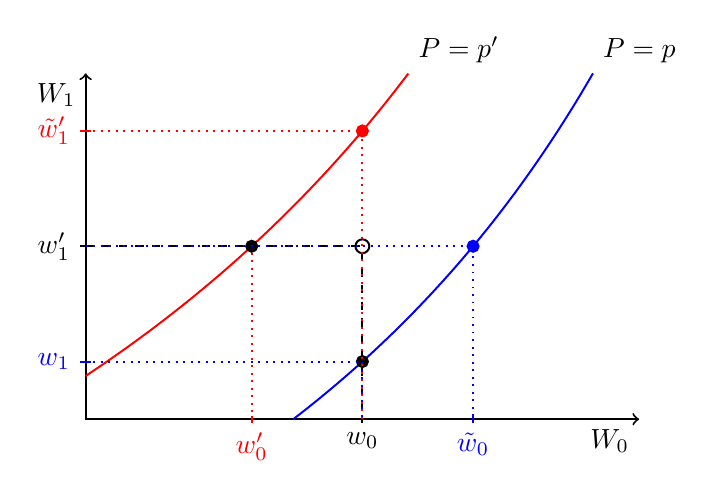
\begin{tikzpicture}[x=200pt,y=125pt, line width=0.25mm] 
\draw[<->](0,1)--(0,0)--(1,0); 
% P = 0.55; xmin=max(0, (P-0.5)/(-0.4)); xmax = min(1, (P-0.5-0.4)/(-0.2-0.4))
\draw[scale=1, domain=0:(0.55-0.5-0.4)/(-0.2-0.4), smooth, variable=\x, red] plot ({\x}, {(0.55-0.5+0.4*\x)/(0.4-0.2*\x)});
\draw[scale=1, domain=(0.35-0.5)/(-0.4):(0.35-0.5-0.4)/(-0.2-0.4), smooth, variable=\x, blue] plot ({\x}, {(0.35-0.5+0.4*\x)/(0.4-0.2*\x)});
%\draw (0.5, 0.5) node{+};
%\filldraw[black] (0.5,0.5) circle (2.5pt);
\draw[black] (0.5,0.5) circle (2.5pt);
%\filldraw[black] (0,0.5) cross (2pt) node[left]{$w_1$};
% w0, w1
\draw (0.01, 0.5) -- (-0.01, 0.5) node[left=0pt]{$w_1'$};
\draw (0.5, 0.01) -- (0.5, -0.01) node[below=0pt]{$w_0$};
\draw[dashed](0,0.5)--(0.5,0.5)--(0.5,0);
% All the other points: %(P-0.5+0.4*0.5)/(0.4-0.2*0.5)
\filldraw[red] (0.5,0.55/0.3-1) circle (2pt);
\filldraw[black] (0.5,0.35/0.3-1) circle (2pt);
\draw [red] (0.01, 0.55/0.3-1) -- (-0.01, 0.55/0.3-1) node[left=0pt, red]{$\tilde{w}_1'$};
\draw [blue] (0.01, 0.35/0.3-1) -- (-0.01, 0.35/0.3-1) node[left=0pt, blue]{$w_1$};
\draw[dotted, blue](0,0.35/0.3-1)--(0.5,0.35/0.3-1)--(0.5,0);
\draw[dotted, red](0,0.55/0.3-1)--(0.5,0.55/0.3-1)--(0.5,0);
% (P-0.5-0.4*0.5)/(-0.4-0.2*0.5)
\filldraw[black] (-0.55/0.5+1.4,0.5) circle (2pt);
\filldraw[blue] (-0.35/0.5+1.4,0.5) circle (2pt);
\draw [red] (-0.55/0.5+1.4, 0.01) -- (-0.55/0.5+1.4, -0.01) node[below=0pt, red]{$w_0'$};
\draw [blue] (-0.35/0.5+1.4, 0.01) -- (-0.35/0.5+1.4, -0.01) node[below=0pt, blue]{$\tilde{w}_0$};
\draw[dotted, red](0, 0.5)--(-0.55/0.5+1.4, 0.5)--(-0.55/0.5+1.4, 0);
\draw[dotted, blue](0, 0.5)--(-0.35/0.5+1.4, 0.5)--(-0.35/0.5+1.4, 0);
\draw (0, 1) node[below left=0pt, black]{$W_1$};
\draw (1, 0) node[below left=0pt, black]{$W_0$};
\draw (-0.35/0.6+1.5, 1) node[above right=0pt, black]{$P=p$};
\draw (-0.55/0.6+1.5, 1) node[above right=0pt, black]{$P=p'$};
\end{tikzpicture} 
\caption{Identification of $\Delta_{LATE}(w_0, w_1', p, p')$ with two iso-probability curves}\label{fig_late_identification}
\end{center}
\end{figure}

\indent For a general $(w_0, w_1', p, p')$, the identification of $\Delta_{LATE}(w_0, w_1', p, p')$ requires the existence of four specific points, two on the isocurve of probability $p'$ and two on the isocurve of probability $p$, as displayed in Figure \ref{fig_late_identification}. Two points are needed on each isocurve to isolate the effect of the semi-IVs on their respective potential outcomes at $P=p$ or $P=p'$. \\ %\\
\indent Notice also that the entire proof to derive (\ref{eq_late_identified}) can be adapted if $P(z)=p > P(z')=p'$. In this case, under uniformity $D(z')-D(z)$ is only equal to zero or $-1$ if $D(z')=0$ and $D(z)=1$, and the set of compliers are individuals who switch out of treatment, from $D=1$ to $D=0$, when one exogenously changes $Z$ from $z$ to $z'$. The formula (\ref{eq_late_identified}) naturally adapts with a minus sign. As a consequence, the Statement (i) of the Theorem \ref{theorem_late} can be adapted for $p < p'$, if one generally redefines, 
\begin{align*}
	\Delta_{LATE}(z, z') = \mathbb{E}[ \ Y_1(w_1') - Y_0(w_0) \ | \ \text{Compliers}(z, z') \ ],
\end{align*}
with the compliers being defined as the individuals with $D(z')=0$ and $D(z)=1$ if $p > p'$ and with $D(z')=1, D(z)=0$ otherwise.  \\
\indent The second definition of the LATE, $\Delta_{LATE}(w_0, w_1', p, p')$, is more general because it does not depend on specific $z, z'$. Thus, if the four points defined previously exist (as in Figure \ref{fig_late_identification}), and if $P(z)=p > P(z')=p'$, then we still identify $\Delta_{LATE}(w_0, w_1', p', p)$ according to Statement (ii) and (iii) of the Theorem \ref{theorem_late}.  Indeed, since $w_0 \in \mathcal{I}_{W_0}(p)\cap\mathcal{I}_{W_0}(p')$ and $w_1' \in \mathcal{I}_{W_1}(p)\cap\mathcal{I}_{W_1}(p')$, if $P(z')=p' < P(z)=p$, one can simply redo all the analysis by comparing $\tilde{z}=(w_0, \tilde{w}_1')$ to $\tilde{z}'=(\tilde{w}_0, w_1')$, instead of $z$ to $z'$. In this case, $P(\tilde{z}')=\tilde{p}'=p > P(\tilde{z})=\tilde{p}=p'$, so we fall back into the previous analysis with $\tilde{p}' > \tilde{p}$.\footnote{Indeed, one can show that $\mathbb{E}\big[ Y | Z=\tilde{z}' \big] - \mathbb{E}\big[ Y | Z=\tilde{z} \big] = \mathbb{E}\big[ (Y_1(w_1') - Y_0(w_0)) ( D(\tilde{z}') - D(\tilde{z}) ) \big]  + \mathbb{E}\big[ (Y_0(\tilde{w}_0) - Y_0(w_0)) (1-D(\tilde{z}')) \big] + \mathbb{E}\big[ (Y_1(w_1') - Y_1(\tilde{w}_1')) D(\tilde{z}) \big].$ Since $P(\tilde{z}')=P(z)=p$ and $P(\tilde{z})=P(z')=p'$, $D(\tilde{z}') = D(z)$ and $D(\tilde{z})=D(z')$, $\mathbb{E}\big[ (Y_1(w_1') - Y_0(w_0)) ( D(\tilde{z}') - D(\tilde{z}) ) \big] = \Delta_{LATE}(w_0, w_1', p', p) (p-p')$. Then to identify it, we first identify the effect of $W_0$ on $Y_0$ at $P=p$ using $z=(w_0, w_1)$, and the effect of $W_1$ on $Y_1$ at $P=p'$ using $z'=(w_0', w_1')$. }  \\
%
%
%
\indent About the exclusion restriction, the necessary condition for identification is, again, that for each alternative, we need at least one excluded semi-IV, and thus, several semi-IVs overall. % not exactly true, cf the conditional IV case...
Otherwise, we would not have variations such that at any given $w_0$ (or $w_1'$) we observe different selection probabilities, and observing several $p$ for a given $w_0$ (and several $w_0$ for a given $p$) is necessary to identify and control for the effect of the semi-IVs on the potential outcomes from which they are not excluded. In other words, thanks to the partial exclusion, for any $(w_0, w_1')$, $\mathcal{P}_{W_0}(w_0)$ and $\mathcal{P}_{W_1}(w_1')$ can be more than a singleton, and this is the main necessary condition for identification. % If they are a singleton, Theorem 3 cannot be satisfied because there is only one p (and thus no p'), in the union of the two sets
At any given $w_0$ and $w_1'$, in addition to them not being a singleton, we want the support of observable selection probabilities, i.e., $\mathcal{P}_{W_0}(w_0)$ and $\mathcal{P}_{W_1}(w_1')$, to be as large as possible. The largest these are, the larger the set of identified LATEs at any given $(w_0, w_1')$. This is a relevance condition on the effect of the semi-IVs on the selection probabilities.\footnote{Notice that, at a given observable effect on the selection (i.e., at given $p'-p$), the set of LATEs that can be identified using semi-IVs is smaller than the one that can be identified using standard IVs because of the additional restrictions on $w_0$ and $w_1'$. In practice, however,  IVs are harder to find than semi-IVs. Thus, despite the stronger relevance requirement, the set of LATEs (in terms of $p, p'$) identifiable with semi-IVs may still be larger than the one identifiable with fewer IVs.} \\
\indent Since for any $(w_0, w_1)$, $P(w_0, w_1)$ are observed in the data, we know $\mathcal{P}_{W_0}(w_0)$ and $\mathcal{P}_{W_1}(w_1')$, and thus we know which LATEs can be identified with the semi-IVs. The relevance condition to obtain identification is not necessarily too restrictive, depending on the model and the type of semi-IVs. By construction, if we only have semi-IVs with limited support (e.g., binary semi-IVs), the relevance condition is hard to satisfy, since we rarely have several combinations of semi-IVs yielding the same selection probability. However, with continuous semi-IVs, we can identify a large set of LATEs. 
\noindent In general, ceteris paribus, the more relevant the semi-IVs (i.e., the larger the impact of the semi-IVs on the selection probabilities and the larger the support $\mathcal{P}_{W_d}(p)$ for any $d$ and $p$), the larger the set of identifiable LATEs from the data.\footnote{Here, there is no restriction on the effect of the semi-IVs on their potential outcomes. If we impose additional assumptions, such as additive separability of the semi-IVs with respect to the shocks $\Eta_0$ and $\Eta_1$ in the potential outcome equations, the relevance condition would be weaker than the current definition of $\mathcal{P}_{W_d}$, and the set of identified LATEs would be larger.} \\ 
\indent Let me illustrate how to check what the identified set of LATEs is a priori, using the selection probabilities observed in the data in two examples.  \\ 
%
%
%

\noindent \textit{Identified LATEs with two binary semi-IVs:} \\ 
Imagine we have two binary semi-IVs, $(W_0, W_1) \in \{0, 1\}^2$, i.e., only four points in the support of the semi-IVs: $(0,0), (0,1), (1,0), (1,1)$. This strongly limits the possibilities to identify the local effect of the semi-IVs on their potential outcomes. %separately from the effect of the semi-IVs on the selection. 
In this case, according to Theorem \ref{theorem_late}, the identification of the LATE requires that at least two of the four selection probabilities are equal, and more specifically, that either $P(1,0) = P(0,1)$ or $P(0,0) = P(1,1)$. 
If $P(1,0) = P(0,1)=\tilde{p}$, for $(w_0, w_1') = (1,1)$, one can identify $\Delta_{LATE}(1,1, P(1,1), \tilde{p})$ if $\tilde{p} > P(1,1)$, or $\Delta_{LATE}(1,1, \tilde{p}, P(1,1))$ if $\tilde{p} < P(1,1)$.
For $(w_0, w_1') = (0,0)$, one can identify $\Delta_{LATE}(0,0, P(0,0), \tilde{p})$ if $\tilde{p} > P(0,0)$, or $\Delta_{LATE}(0,0, \tilde{p}, P(0,0))$ if $\tilde{p} < P(0,0)$. 
Similarly, if $P(0,0) = P(1,1)=p'$, one can identify $\Delta_{LATE}(0,1, P(0,1), p')$ (or $\Delta_{LATE}(0,1, p', P(0,1))$) for $(w_0, w_1') = (0,1)$, and $\Delta_{LATE}(1,0, P(1,0), p')$ (or $\Delta_{LATE}(1,0, p', P(1,0))$) for $(w_0, w_1') = (1,0)$. %\\
Thus, in general, with two binary semi-IVs, the identification of the LATE is limited to very specific cases, and we will generally prefer to have continuous semi-IVs to identify LATEs. The limitations on identification come from the limited support, regardless of how strong of an impact the semi-IVs have on the selection probabilities.  \\










\begin{figure}[!h]
\begin{center}
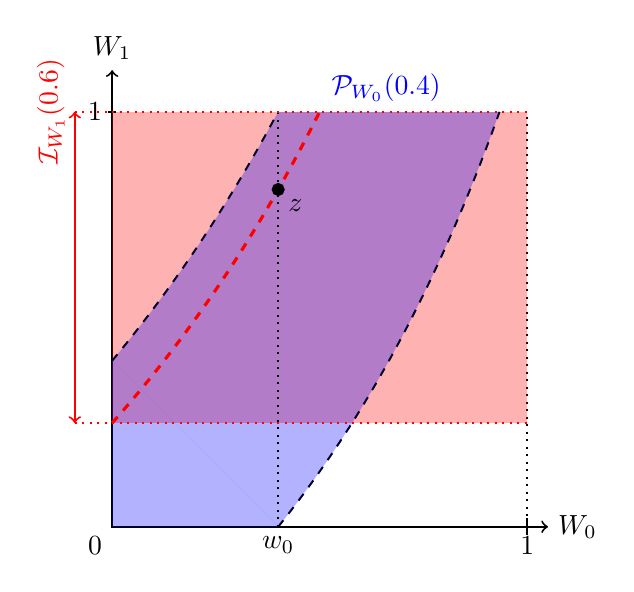
\begin{tikzpicture}[x=150pt,y=150pt, line width=0.25mm] 
\draw[<->](0,1.1)--(0,0)--(1.05,0); 
\draw[-, dotted](0,1)--(1,1)--(1,0);
\fill [red, semitransparent, opacity=0.3] (0, 0.25) rectangle (1, 1); 
\draw[name path=min, scale=1, dashed, domain=(0.34-0.5)/(-0.4):(0.34-0.5-0.4)/(-0.2-0.4), smooth, variable=\x, black] plot ({\x}, {(0.34-0.5+0.4*\x)/(0.4-0.2*\x)});
\draw[name path=max, scale=1, dashed, domain=0:(0.66-0.5-0.4)/(-0.2-0.4), smooth, variable=\x, black] plot ({\x}, {(0.66-0.5+0.4*\x)/(0.4-0.2*\x)});
\tikzfillbetween[of=min and max]{blue, opacity=0.3} 
% Need to correct for the domain difference:
\fill[blue, opacity=0.3] (0,0)--(0.4, 0)--(0, 0.16/0.4);
% Place the baseline point z:
\draw[name path=baseline, scale=1, dashed, line width=0.4mm, domain=0:(0.6-0.5-0.4)/(-0.2-0.4), smooth, variable=\x, red] plot ({\x}, {(0.6-0.5+0.4*\x)/(0.4-0.2*\x)});
%\tikzfillbetween[of=baseline and max]{soft clip={domain=1:3}, split, every segment no 0/.style={pattern=north east lines,pattern color=gray}} 
%\tikzfillbetween[of=baseline and max]{magenta, opacity=0.3} 
\filldraw[black] (0.4,0.8125) circle (2pt) node[below right=0pt]{$z$};
\draw[-, dotted, black](0.4, 0)--(0.4, 1); 
\draw (0.4, 0) node[below=0pt, black]{$w_0$};
% Sets:
\draw[<->, red] (-0.09,0.6/0.4-0.5/0.4) -- (-0.09,1) node[above, rotate=90]{$\mathcal{I}_{W_1}(0.6)$};; 
% Identification square:
\draw (0, 1.1) node[above=0pt, black]{$W_1$};
\draw (1.05, 0) node[right=0pt, black]{$W_0$};
\draw (1, 0) node[below=0pt, black]{$1$};
\draw (1,0.02) -- (1,-0.02);
\draw (0, 1) node[left=0pt, black]{$1$};
\draw (0.01, 1) -- (-0.01, 1);
\draw (0, 0) node[below left=0pt, black]{$0$};
\draw (0.66, 1) node[above=0pt, blue]{$\mathcal{P}_{W_0}(0.4)$};
%\draw (-0.34/0.6+1.5, 1) node[above=0pt, black]{$p=\underline{p}$};
%\draw (-0.66/0.6+1.5, 1) node[above=0pt, black]{$p=\bar{p}$};
\draw[-, dotted, red](-0.09, 0.25)--(1, 0.25); 
\draw[-, dotted, red](-0.09, 1)--(1, 1);  
\end{tikzpicture} 
\subcaption{Set of $z'$ for which $\Delta_{LATE}(z, z')$ is identified, with $z=(0.4, 0.8125)$}\label{fig_late_example2}
 %, starting from $w_0=0.4$ and $p=0.6$ \\(i.e., $z=(0.4, 0.8125)$, $P(z)=0.6$).}
\end{center}

\begin{center}
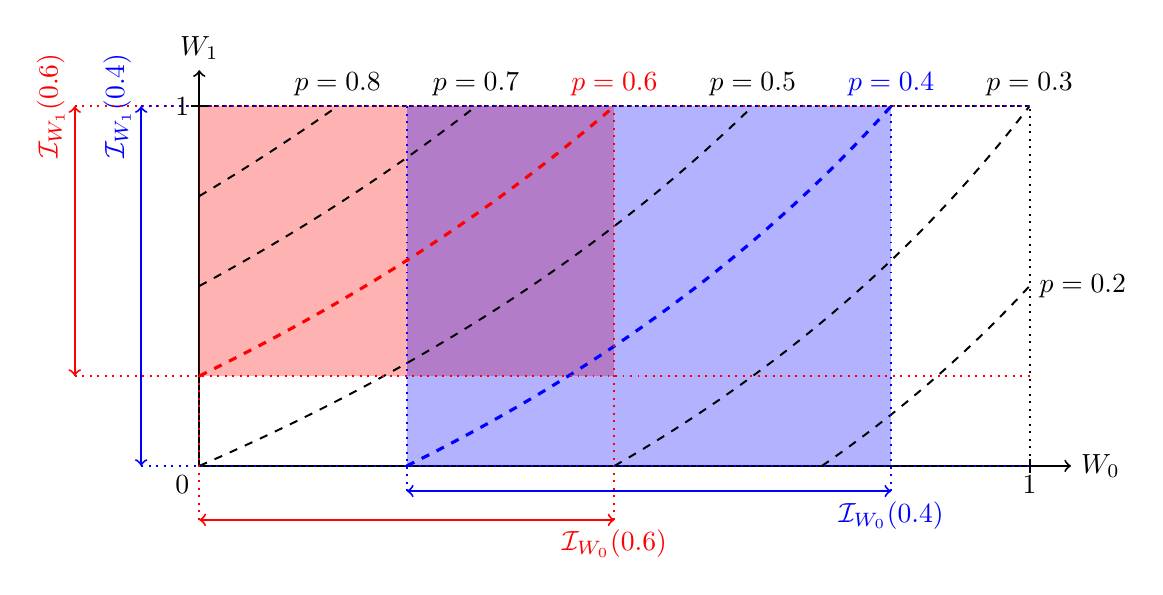
\begin{tikzpicture}[x=300pt,y=130pt, line width=0.25mm] 
\draw[<->](0,1.1)--(0,0)--(1.05,0); 
\draw[-, dotted](0,1)--(1,1)--(1,0);
%\fill [yellow] (-0.4/0.4+0.5/0.4, 0.6/0.4-0.5/0.4) rectangle (-0.6/0.6+0.9/0.6, 1); 
\fill [red, semitransparent, opacity=0.3] (0, 0.6/0.4-0.5/0.4) rectangle (-0.6/0.6+0.9/0.6, 1); 
\fill [blue, semitransparent, opacity=0.3] (-0.4/0.4+0.5/0.4, 0) rectangle (-0.4/0.6+0.9/0.6, 1); 
%\fill [yellow, semitransparent] (-0.4/0.4+0.5/0.4, 0.6/0.4-0.5/0.4) rectangle (-0.6/0.6+0.9/0.6, 1); 
% P = 0.55; xmin=max(0, (P-0.5)/(-0.4)); xmax = min(1, (P-0.5-0.4)/(-0.2-0.4))
\draw[scale=1, dashed, domain=(0.2-0.5)/(-0.4):1, smooth, variable=\x, black] plot ({\x}, {(0.20-0.5+0.4*\x)/(0.4-0.2*\x)});
\draw[scale=1, dashed, domain=(0.3-0.5)/(-0.4):1, smooth, variable=\x, black] plot ({\x}, {(0.30-0.5+0.4*\x)/(0.4-0.2*\x)});
\draw[scale=1, line width=0.4mm, dashed, domain=(0.4-0.5)/(-0.4):(0.40-0.5-0.4)/(-0.2-0.4), smooth, variable=\x, blue] plot ({\x}, {(0.40-0.5+0.4*\x)/(0.4-0.2*\x)});
\draw[scale=1, dashed, domain=0:(0.50-0.5-0.4)/(-0.2-0.4), smooth, variable=\x, black] plot ({\x}, {(0.50-0.5+0.4*\x)/(0.4-0.2*\x)});
\draw[scale=1, dashed, line width=0.4mm, domain=0:(0.60-0.5-0.4)/(-0.2-0.4), smooth, variable=\x, red] plot ({\x}, {(0.60-0.5+0.4*\x)/(0.4-0.2*\x)});
\draw[scale=1, dashed, domain=0:(0.70-0.5-0.4)/(-0.2-0.4), smooth, variable=\x, black] plot ({\x}, {(0.70-0.5+0.4*\x)/(0.4-0.2*\x)});
\draw[scale=1, dashed, domain=0:(0.80-0.5-0.4)/(-0.2-0.4), smooth, variable=\x, black] plot ({\x}, {(0.80-0.5+0.4*\x)/(0.4-0.2*\x)});
% Sets:
\draw[<->, blue](-0.07,0)--(-0.07,1) node[above, rotate=90]{$\mathcal{I}_{W_1}(0.4)$};
%\draw (-0.07,0.5)  node[above, blue, rotate=90]{$\mathcal{I}_{W_0}(0.4)$}; 
\draw[<->, red] (-0.15,0.6/0.4-0.5/0.4) -- (-0.15,1) node[above, rotate=90]{$\mathcal{I}_{W_1}(0.6)$};; 
%\draw (-0.15,0.5+0.6/0.8-0.5/0.8)  node[above, red, rotate=90]{$\mathcal{I}_{W_1}(0.6)$};
\draw[<->, blue](-0.4/0.4+0.5/0.4,-0.07)--(-0.4/0.6+0.9/0.6,-0.07) node[below]{$\mathcal{I}_{W_0}(0.4)$};
\draw[<->, red](0,-0.15)--(-0.6/0.6+0.9/0.6,-0.15) node[below]{$\mathcal{I}_{W_0}(0.6)$};
% Identification square:
\draw[-, dotted, red](0,-0.15)--(0, 0.6/0.4-0.5/0.4); 
\draw[-, dotted, red](-0.6/0.6+0.9/0.6,-0.15)--(-0.6/0.6+0.9/0.6,1); 
\draw[-, dotted, blue](-0.4/0.4+0.5/0.4,-0.07)--(-0.4/0.4+0.5/0.4, 1); 
\draw[-, dotted, blue](-0.4/0.6+0.9/0.6,-0.07)--(-0.4/0.6+0.9/0.6,1); 
\draw[-, dotted, red](-0.15,0.6/0.4-0.5/0.4)--(1, 0.6/0.4-0.5/0.4); 
\draw[-, dotted, red](-0.15,1)--(1,1); 
\draw[-, dotted, blue](-0.07,0)--(1, 0); 
\draw[-, dotted, blue](-0.07,1)--(1,1); 
\draw (0, 1.1) node[above=0pt, black]{$W_1$};
\draw (1.05, 0) node[right=0pt, black]{$W_0$};
\draw (1, 0) node[below=0pt, black]{$1$};
\draw (1,0.02) -- (1,-0.02);
\draw (0, 1) node[left=0pt, black]{$1$};
\draw (0.01, 1) -- (-0.01, 1);
\draw (0, 0) node[below left=0pt, black]{$0$};
\draw (1, 0.20/0.2 - 0.1/0.2) node[right=0pt, black]{$p=0.2$};
\draw (-0.30/0.6+1.5, 1) node[above=0pt, black]{$p=0.3$};
\draw (-0.40/0.6+1.5, 1) node[above=0pt, blue]{$p=0.4$};
\draw (-0.50/0.6+1.5, 1) node[above=0pt, black]{$p=0.5$};
\draw (-0.60/0.6+1.5, 1) node[above=0pt, red]{$p=0.6$};
\draw (-0.70/0.6+1.5, 1) node[above=0pt, black]{$p=0.7$};
\draw (-0.80/0.6+1.5, 1) node[above=0pt, black]{$p=0.8$};
%\draw (1, 0.20/0.2 - 0.1/0.2) node[above=0pt, black, rotate=55]{$p=0.2$};
%\draw (-0.30/0.6+1.5, 1) node[above=0pt, black, rotate=60]{$p=0.3$};
%\draw (-0.40/0.6+1.5, 1) node[above=0pt, blue, rotate=55]{$p=0.4$};
%\draw (-0.50/0.6+1.5, 1) node[above=0pt, black, rotate=50]{$p=0.5$};
%\draw (-0.60/0.6+1.5, 1) node[above=0pt, red, rotate=45]{$p=0.6$};
%\draw (-0.70/0.6+1.5, 1) node[above=0pt, black, rotate=45]{$p=0.7$};
%\draw (-0.80/0.6+1.5, 1) node[above=0pt, black, rotate=45]{$p=0.8$};
%\fill [orange] (0.1,0.1) rectangle (0.2,0.2);
\end{tikzpicture} 
\subcaption{Set of $(w_0, w_1')$ for which $\Delta_{LATE}(w_0, w_1', 0.4, 0.6)$ is identified.}\label{fig_late_example}
\end{center}
\caption{Identified sets of LATEs}\label{fig_late_example_general}
\end{figure}








\noindent \textit{Identified LATEs with continuous semi-IVs:} \\ 
As soon as we have two (or more) continuous semi-IVs, we can naturally identify a large set of LATEs.  
Imagine we have two continuous semi-IVs, $(W_0, W_1) \in [0, 1]^2$. For the illustration, suppose the selection equation is simple and yields $P(w_0, w_1) = \delta + \delta_0 w_0 + \delta_1 w_1 + \delta_2 w_0 w_1$. This is the example illustrated in Figure \ref{fig_late_example_general}, with $\delta, \delta_0, \delta_1, \delta_2$ equal to $0.5, -0.4, 0.4$ and $-0.2$, respectively. In the example of returns to college, $W_0$ and $W_1$ are the (continuous and normalized) local average earnings of college-non-goers and college-goers, and we may have this type of selection equation since higher $W_0$ means higher earnings expectations if one does not go to college, and hurts the probability of going to college, while better earnings expectations after college ($W_1$) increase the probability of going. \\
\indent A first question is to determine which LATEs can be identified, starting from a given $z=(w_0, w_1)$, with $P(z)=p$. In this case, $\Delta_{LATE}(z, z')$ will be identified for any $z'=(w_0', w_1')$ with $P(z')=p'$ such that $w_1' \in \mathcal{I}_{W_1}(p)$, $p' \in \mathcal{P}_{W_0}(w_0)$, and $p' > p$. If we extend the definition of $\Delta_{LATE}(z, z')$ to be the effect on compliers but allowing for $p > p'$ (in which case the compliers are the ones who switch out of treatment when $Z$ goes from $z$ to $z'$), we identify the LATE for any $z'=(w_0', w_1')$ such that $w_1' \in \mathcal{I}_{W_1}(p)$ and $P(z') \in \mathcal{P}_{W_0}(w_0)$. In the example of Figure \ref{fig_late_example2} with $w_0=0.4$ and $P(w_0, w_1)=0.6$ (which implies $w_1=0.8125$ here), it means that we identify LATEs for any $z'$ in the large purple area. If we restrict ourselves to $z'$ for which $p'>p$, one only identifies the LATEs in the purple area above the isocurve of probability $P(z)=p=0.6$ (the dashed red curve). \\
\indent One may also wonder, given $p$ and $p'$, for which $(w_0, w_1')$ can $\Delta_{LATE}(w_0, w_1', p, p')$ be identified. For example, following Figure \ref{fig_late_example}, between $p=0.4$ and $p'=0.6$, one can identify $\Delta_{LATE}(w_0, w_1', 0.4, 0.6)$ for any $w_0 \in \mathcal{I}_{W_0}(0.4)\cap\mathcal{I}_{W_0}(0.6)$ and $w_1' \in \mathcal{I}_{W_1}(0.4)\cap\mathcal{I}_{W_1}(0.6)$, i.e., for any $(w_0, w_1')$ in the purple area, which is quite large. %\\
In both figures, \ref{fig_late_example2} and \ref{fig_late_example}, the purple area is the area in which we can identify the effect of the semi-IVs on their respective potential outcomes, and thus identify the LATE. \\
\indent As for the MTEs at probability $p$, with continuous semi-IVs with regular effect on the selection probabilities, they are naturally identified for any $(w_0, w_1')$ on the isocurve of probability $p$. 






















\section{Average treatment effect in an additive model with homogenous treatment effect}\label{section_ate}
\subsection{Identification}\label{subsection_ate_identification}

In a simple additive model with a homogenous treatment effect, the ATE is identified and has a simple closed-form formula. 
This provides the intuition needed to understand the identification with semi-IVs in the nonseparable model with rank invariance, and can also be used in practice to build easy-to-implement estimators of treatment effects with semi-IVs. 
Again, I abstract from covariates $X$ for the identification (everything is conditional on $X=x$), but they can be trivially included. \\
\indent Focus again on the example with two binary semi-IVs, $W_0$ and $W_1$ (though the following arguments are easily extended to continuous semi-IVs). Imagine the potential outcomes have the following form, with additive $\Eta$:
\begin{align}\label{model_simple}
	&Y = \beta + \delta D + \alpha_0 (1-D) W_0 + \alpha_1 D W_1 + \Eta \\
	\quad \text{ with } \quad &\mathbb{E}[\Eta | W_0=w_0, W_1=w_1] = 0 \text{ for all } (w_0, w_1) \in \{0, 1\}^2. \nonumber
\end{align}
The only assumption is really that $\Eta$ is additively separable. Otherwise, we generally have four unknown quantities to identify: $\mathbb{E}[Y_0 | W_0 = 0],  \mathbb{E}[Y_0 | W_0 = 1], \mathbb{E}[Y_1 | W_1 = 0],$ and $\mathbb{E}[Y_1 | W_1 = 1]$, where $Y_0$ and $Y_1$ are the unknown potential outcomes. There is a one-to-one mapping between these quantities and the four parameters $\beta, \delta, \alpha_0,$ and $\alpha_1$ in the specification. 
We change the normalization and now assume that $\Eta$ has mean zero (instead of $\Eta \sim \mathcal{U}(0,1)$). With the additivity of $\Eta$, we still have monotonicity of $Y_d$ with respect to $\Eta$ and we also have rank invariance: ceteris paribus, the higher $\Eta$, the higher $Y$. 
\noindent Notice that here, the ATE is homogenous (given $w_0, w_1$), but not limited to $\delta$. It is:
\begin{align*}
	ATE = \mathbb{E}[Y_1 - Y_0] = \delta + \alpha_1 \mathbb{E}[W_{1}] - \alpha_0 \mathbb{E}[W_{0}], 
\end{align*} 
In other words, because of the partial exclusion restrictions, the average values of the semi-IVs also enter the average treatment effect. One could alternatively define conditional $ATE(w_0, w_1)$, i.e., the ATE at specific values of the semi-IVs instead. \\
%
%
%
%
\indent In terms of identification, since $\mathbb{E}[\Eta | W_0=w_0, W_1=w_1] = 0$, for all $(w_0, w_1) \in \{0,1\}^2$, we have:
\begin{align}\label{eq_ATE}
	\mathbb{E}[Y | W_0=w_0, W_1=w_1] = &\quad \beta + \delta \textrm{Pr}(D=1|W_0=w_0, W_1=w_1) \nonumber \\
	&+ \alpha_0 w_0 \textrm{Pr}(D=0|W_0=w_0, W_1=w_1) \nonumber \\
	&+ \alpha_1 w_1 \textrm{Pr}(D=1|W_0=w_0, W_1=w_1).
\end{align}
Denote $p_{D|w_0, w_1}(1) = \textrm{Pr}(D=1|W_0=w_0, W_1=w_1)$. Since $p_{D|w_0, w_1}(1) = 1-p_{D|w_0, w_1}(0)$, we can rewrite (\ref{eq_ATE}) as: \\
%
\begin{align}\label{system_ATE}
\begin{bmatrix}
	\mathbb{E}[Y | W_0=0, W_1=0] \\
	\mathbb{E}[Y | W_0=1, W_1=0] \\
	\mathbb{E}[Y | W_0=0, W_1=1] \\
	\mathbb{E}[Y | W_0=1, W_1=1]
\end{bmatrix} = 
	\underbrace{\begin{bmatrix}
		1 & p_{D|0, 0}(1) & 0 & 0 \\
		1 & p_{D|1, 0}(1) & 1- p_{D|1, 0}(1)& 0\\
		1 & p_{D|0, 1}(1) & 0 & p_{D|0, 1}(1)\\
		1 & p_{D|1, 1}(1) & 1- p_{D|1, 1}(1)& p_{D|1, 1}(1)\\
	\end{bmatrix}}_{:= A}
	\begin{bmatrix}
		\beta \\
		\delta \\
		\alpha_0 \\
		\alpha_1 
	\end{bmatrix}.
\end{align}
Thus, if $A$ is invertible, we have a closed-form formula for the coefficients given by
\begin{align}\label{solution_ATE}
	\begin{bmatrix}
		\beta \\
		\delta \\
		\alpha_0 \\
		\alpha_1 
	\end{bmatrix} = A^{-1} \begin{bmatrix}
	\mathbb{E}[Y | W_0=0, W_1=0] \\
	\mathbb{E}[Y | W_0=1, W_1=0] \\
	\mathbb{E}[Y | W_0=0, W_1=1] \\
	\mathbb{E}[Y | W_0=1, W_1=1]
\end{bmatrix}. 
\end{align}
Now, 
\begin{align*}
	\text{det}(A) = &\quad p_{D|0, 0}(1) p_{D|1, 1}(1) (1-p_{D|0, 1}(1))(1-p_{D|1, 0}(1)) \\
	&- p_{D|0, 1}(1) p_{D|1, 0}(1) (1-p_{D|0, 0}(1))(1-p_{D|1, 1}(1)),
\end{align*}
and det($A$)$=0$ if and only if
\begin{align*}
	\frac{p_{D|0, 0}(1)/(1-p_{D|0, 0}(1))}{p_{D|0, 1}(1)/(1-p_{D|0, 1}(1))} = \frac{p_{D|1, 0}(1)/(1-p_{D|1, 0}(1))}{p_{D|1, 1}(1)/(1-p_{D|1, 1}(1))}. 
\end{align*}
This is the same odds ratio condition as the relevance condition (\ref{irrelevant_odds}) in Section \ref{section_framework}, except that this time it is a condition on the overall probabilities (not conditional on $\Eta$). So, the intuition behind the identification of the ATE is the same as the intuition behind the identification of the general nonseparable model with rank invariance. 





\subsection{Estimation} 

I build a `semi-IV GMM' estimation procedure, naturally extending IV GMM to semi-IVs, to estimate the additive model (\ref{model_simple}) of the previous sub-section \ref{subsection_ate_identification}, with covariates that also enter additively. We allow for discrete $D \in \{1, \hdots, J\}$, thus we observe an outcome $Y = \sum_d^{J} \mathds{1}\{ D=d\} Y_d$. For each alternative $d$, denote $W_d$, the $N\times N_{W_d}$ matrix of $N_{W_d}$ semi-IVs which are non-excluded from the potential outcome $Y_d$.\footnote{As explained in Section \ref{section_generalization} and in the examples in Appendix \ref{appendix_example_exclusion}, there may be some variables which are not excluded from several potential outcomes, as long as they are excluded from some of them, they are still valid semi-IVs.} The semi-IVs can be binary, discrete, or even continuous variables and we generally allow for multiple semi-IVs per alternative. Also, denote as $X$ the standard (non-excluded) covariates. We have a sample of $N$ observations and we want to estimate: 
\begin{align}\label{model_estimate} &Y = \mathbf{X} \beta + \Eta, \\ 
%\text{with } \quad &\mathbb{E}[\Eta | \mathbf{Z}] = 0, \nonumber
\text{with } \quad &\mathbb{E}[\mathbf{Z}\Eta] = 0, \nonumber
\end{align} 
where $\mathbf{X}$ is the general set of covariates for which we want to estimate the effect on $Y$, and $\mathbf{Z}$ is a matrix of `instruments'.  %\\
The general covariates $\mathbf{X}$ are defined as, 
\begin{align*}
	\mathbf{X} = \Bigg[ \overbrace{\underset{(N\times K)}{X}}^{\text{covariates}} \quad  \overbrace{ \underset{(N\times 1)}{\mathds{1}_{\{D=2\}}} \quad \hdots \quad \underset{(N\times 1)}{\mathds{1}_{\{D=J\}}}}^{\text{endogenous variables}}  \quad \overbrace{\underbrace{\underset{(N\times N_{W_1})}{\mathds{1}_{\{D=1\}} W_1}\quad \hdots \quad \underset{(N\times N_{W_J})}{\mathds{1}_{\{D=J\}} W_J}}_{(N\times \sum_d N_{W_d})}}^{\text{semi-IVs (interacted with $D$)}} \quad \Bigg].
\end{align*}
The general set of covariates, $\mathbf{X}$, includes the standard exogenous covariates $X$ (including a constant), and the endogenous discrete variable $D$ that I split into $J$ binary variables to have one effect per alternative with $\mathbb{E}[D | \Eta] \neq 0$. The intercept included in $X$ will capture the baseline effect when $D=1$, and the coefficients associated with the other dummies represent deviations from this baseline. The general set of covariates $\mathbf{X}$ also includes other endogenous variables: the semi-IVs interacted with the discrete endogenous variable, where we only included the interaction of $W_d$ with $D=d$ for each $d$.\footnote{An equivalent way to write (\ref{model_estimate}) is: \begin{align*}
	Y_d = X\beta_x \ + \ \delta_d \ + W_d \alpha_d \ + \ \Eta \quad \text{for each } d \in \{1, ..., J\}.  \end{align*}} \\ 
\indent To control for the endogenous variable, the matrix of instruments, $\mathbf{Z}$, is given by 
\begin{align*}
	\mathbf{Z} = [ X \quad W_1 \quad \hdots \quad W_J \quad L ],
\end{align*}
where $L$ is a $N \times N_L$ matrix of all the interactions/combinations between all the semi-IVs (i.e., $N_L = \prod_{d \in \{1, ..., J\}} N_{W_d}$), such that each row $r$ of $L$ is given by 
\begin{align*}
	L_{r\cdot} = [W_{1r\cdot} \otimes W_{2r\cdot} \otimes \hdots \otimes W_{Jr\cdot}],
\end{align*}
where $\otimes$ is the Kronecker product of the variables. 
As in the identification proof, the idea is that, not only the semi-IVs, but also their interactions give identification power. Therefore, in general, we include all interaction terms in the set of instruments. The matrix $\mathbf{Z}$ contains $K + \sum_{d \in \{1, ..., J\}} N_{W_d} + \prod_{d \in \{1, ..., J\}} N_{W_d}$ columns (and $N$ rows). \\
%
%
\indent Notice that the endogenous variables are obviously not in the set of exogenous instruments $\mathbf{Z}$. As in the previous sections, the whole identification comes from the fact that there are enough `relevant' interactions between the semi-IVs in $\mathbf{Z}$, which are excluded from $Y$ (due to the partial exclusion restrictions), to estimate the effect of the endogenous variables, $\mathds{1}\{D=d\}$ and $\mathds{1}\{D=d\} W_d$ for all $d$. Obviously, if there are not enough relevant interactions between the semi-IVs (in the sense that the odds ratio condition (\ref{irrelevant_odds}) is violated), or if there is one $d$ for which we do not have a single partial exclusion restriction, the model will not be identified. Generally, with multiple semi-IVs per alternative, the model may be overidentified, as in the corresponding case with multiple IVs.  \\
%
\indent Once the general covariates $\mathbf{X}$ and the set of instruments $\mathbf{Z}$ are defined as explained above, the estimation procedure can follow the standard IV GMM estimation procedure  \citep[cf \texttt{ivreg} in \texttt{Stata},][]{baumetal2003}.  
The estimated coefficients are
\begin{align}\label{est_beta}
	\hat{\beta} &= (\mathbf{X^T}P_Z\mathbf{X})^{-1} \mathbf{X^T} P_Z Y, %\\
	%\text{where} P_Z &= Z(\mathbf{Z'Z})Z'\nonumber
\end{align}
where $P_Z = \mathbf{Z}(\mathbf{Z^TZ})^{-1}\mathbf{Z^T}$ is the projection matrix. Denote the vector of residuals, $\hat{\Eta} = Y - \mathbf{X}\hat{\beta}$. Then, the Eicker-Huber-White sandwich robust variance-covariance matrix of the estimator $\beta$ is given by: 
\begin{align*}
	\text{Robust } V(\hat{\beta}) = (\mathbf{X^T}P_Z\mathbf{X})^{-1} \Big( \mathbf{X^T Z}(\mathbf{Z^T Z})^{-1} \big(\mathbf{Z^T}\hat{\Omega} \mathbf{Z} \big) (\mathbf{Z^T Z})^{-1} \mathbf{Z^T X}\Big) (\mathbf{X^T}P_Z\mathbf{X})^{-1}, 
\end{align*}
where $\hat{\Omega} = \text{diag}\big(\hat{\Eta}_1^2 \cdots \hat{\Eta}_i^2 \cdots \hat{\Eta}_N^2 \big)$ is the $N\times N$ diagonal matrix of all individual residuals. Assuming homoskedasticity instead, we have $V(\hat{\beta}) = \frac{1}{N} \hat{\sigma}^2 (\mathbf{X^T}P_Z\mathbf{X})^{-1}$, where $\hat{\sigma}^2$ is the estimated variance, $\hat{\sigma}^2 = \frac{1}{N} \ \hat{\Eta}^T \hat{\Eta} $.


\subsection{Empirical illustration: returns to college}\label{section_application}


I use the sample of $2,242$ males from the NLSY79 from \cite{heckmanetal2006}, \cite{heckmanetal2016}, \cite{heckmanetal2018}, and which have also been used in \cite{heckmanvytlacil2007a, heckmanvytlacil2007b}, and \cite{carneiroheckmanvytlacil2011} for example.  In addition to their selection (males, non-military, not still in school, and no missing covariates), I also exclude $475$ high school dropouts to study the returns to college for high school graduates, and $100$ observations for which the earnings at age $30$ is not observed. 

I estimate the effect of going to college and receiving at least some college education, $D=1$, instead of stopping education after high school, $D=0$, on earnings of individuals at age $30$, $Y$. %Individuals who dropped out before finishing high school are removed from the sample, while 
College-goers is a broad category that includes individuals who did only `some college' without graduating, bachelor graduates, master graduates, or more highly educated individuals. 
I use semi-IVs related to alternative specific costs and benefits: the education-specific average local (county-level) earnings and unemployment rates, and the local tuition of college (two and four years tuition).  
These variables (taken at age 17), are relatively standard and have been used as instrumental variables to study the returns to college (and GED) in \cite{carneiroheckmanvytlacil2011} and \cite{heckmanvytlacil2007a} for example. However, the exclusion restriction may be debated. Indeed, because of serial correlation in labor market conditions, it is unlikely that one's earnings at $30$ are completely uncorrelated with the average local earnings at $17$ of other individuals with the same level of education. Even if one focuses only on deviations from permanent market conditions, the deviations may persist over time. The partial exclusion restriction imposed on semi-IVs is much weaker and likely to hold. It (only) requires that the past local market conditions of individuals who did not go ($W_0$) do not affect college-goers' earnings at age $30$ (controlling for the past local market conditions of older college-goers, $W_1$).  \\
%
%
\indent Following the previous section, I estimate the linear model
\begin{align*}
	Y = X\beta \ + \ D \delta  \ + (1-D)W_0 \alpha_0 \ + \ DW_1 \alpha_1 + \Eta, 
\end{align*}
and more specifically, the ATE in this model, i.e., 
\begin{align*}
	\text{ATE} &= \mathbb{E}[ Y_1 - Y_0 ] %\\ %\mathbb{E}[Y(D=1, X, W_0, W_1) - Y(D=0, X, W_0, W_1)] \\
	= \mathbb{E}[X\beta + \delta + W_1\alpha_1 - X\beta - W_0\alpha_0] %\\
	= \delta + \mathbb{E}[W_1] \alpha_1 - \mathbb{E}[W_0] \alpha_0. 
\end{align*}
The ATE contains the standard homogenous effect of the endogenous variable ($\delta$), but also the effect of the semi-IVs. \\
%
%
%
%
%
\begin{table}[h!] \centering 
\scalebox{0.9}{
\begin{threeparttable}
  \caption{Returns to education, NLSY79 data}\label{table_education}
\begin{tabular}{@{\extracolsep{5pt}}lcc} 
\\[-1.8ex]\hline 
\hline \\[-1.8ex] 
%& \multicolumn{4}{c}{\textit{Dependent variable:}} \\ 
\cline{2-3} 
\\[-1.8ex] & \multicolumn{2}{c}{log(Earnings) at age $30$} \\ 
\\[-1.8ex] & OLS & semi-IV  \\ 
\hline \\[-1.8ex] 
%  & & & & & \\ 
\textbf{ATE} $= \delta + \mathbb{E}[W_1] \alpha_1 - \mathbb{E}[W_0] \alpha_0$ & 0.242$^{***}$ & 0.185 \\
& (0.023) & (0.241)\\ 
    & & \\  
%    \cline{2-3}  \cline{5-6} \\ 
\textbf{Specification} (for both OLS and semi-IVs) & \multicolumn{2}{c}{semi-IVs} \\
 & \multicolumn{2}{c}{included in:} \\
& $Y_0$ & $Y_1$ \\ 
    \cline{2-3} \\ 
%  & & & & \\ 
Average local earnings of HS & Yes & No \\ 
Local unemployment of HS & Yes & No \\ 
Average local earnings after only Some College & No & Yes \\ 
Average local earnings of Bachelor Graduate & No & Yes \\ 
Local unemployment after only Some College & No & Yes \\
Local unemployment of Bachelor Graduate & No & Yes \\
Local tuition of $2$ years college & No & Yes \\ 
Local tuition of $4$ years college & No & Yes \\  
%&  &  \\ 
& & \\
\hline \\[-1.8ex] 
Observations & \multicolumn{2}{c}{1,667}  \\ 
\hline 
\hline \\[-1.8ex] 
\end{tabular}
\begin{tablenotes}
\small \item\textit{Note:} $^{*}$p$<$0.1; $^{**}$p$<$0.05; $^{***}$p$<$0.01. \\
Two specifications including a different set of semi-IVs. 
The ATE represents the overall effect of education on log(earnings) at age 30. To obtain an effect by year of education, one would need to approximately divide the results by the number of years spent in college (on average about 3). All the semi-IVs are computed locally, at the county level, when the individuals were deciding to go to college or not (at age $17$). The control variables $X$ include race, parents' education, number of siblings, and an indicator of urban residence at age 14. 
\end{tablenotes}
\end{threeparttable}
}	
\end{table}
%%
%
%
\indent The results of the estimation of the ATE using semi-IV GMM are reported in Table \ref{table_education}. I compare them to the estimation of a baseline OLS that does not account for the endogeneity of $D$. The OLS estimates a total return to college of about $24\%$ more earnings at age $30$ on average. Controlling for the endogeneity of education using semi-IVs, the overall effect of education is reduced ($18.5\%$) but non-significant. If it was significant, it would suggest that unobserved ability is biasing the OLS results upward and that students with higher ability select themself more into college. The (robust) standard errors are multiplied by $10$ when using the semi-IVs with respect to the baseline OLS. This is the same order of magnitude as when one uses IVs instead of OLS \citep[cf the survey in][]{card2001}. Notice that I use several semi-IVs per alternative. This is because, if I use only one semi-IV per alternative, for example, only the local earnings of HS and the local earnings of bachelor graduates, these two measures are highly correlated and I do not have a lot of identifying variation left. But these are less correlated with other variables such as tuition and unemployment rates. Thus, these additional semi-IVs introduce additional relevant interactions which reduce the variance of the estimates. \\ 
\indent Finally, note that the estimated results from this `semi-IV GMM' cannot be interpreted as a LATE or as a (positively) weighted sum of several LATEs. But anyway, according to \cite{blandholetal2022}, we would also have lost this interpretation with IVs because we do not include the covariates fully nonparametrically here. 










\section{Conclusion}\label{section_conclusion}

This paper proposes a new tool to address endogeneity problems. I generalize the concept of IVs and show that standard nonparametric identification of models (and treatment effects in models) with discrete endogeneity can still be achieved using only partially excluded semi-IVs. Given the difficulty to find fully excluded IVs in practice, being able to search for semi-IVs instead should have a large empirical impact: it significantly extends the toolkit of applied researchers.  \\
\indent There are several directions for further work. First comes the question of the best way to implement estimation with semi-IVs in practice. In the case of homogenous treatment effect, Section \ref{section_ate} provides a natural 2SLS-like estimator with semi-IVs, which will allow developing packages for most statistical software of interest: the \texttt{semiivreg} equivalent of \texttt{ivreg} in Stata for example. But in the case of heterogeneous treatment effects, one may be interested in more nonparametric approaches: many alternatives are available and need to be studied and further developed. %\\
%
%
\noindent In terms of testing, one can use semi-IVs to test exclusion restrictions imposed on standard IVs: if we can reasonably argue that a variable is excluded from one of the potential outcomes, we can test whether it is also excluded from the others (i.e., if it is an IV) by estimating the model with other semi-IVs and checking whether the estimated effect of the variable on the other potential outcomes is significantly different from zero. Going forward, a natural conservative empirical approach may be to always start with semi-IVs and then test if the partial exclusion restriction can actually be strengthened into a full exclusion restriction. %\\
\noindent The question of what can be identified and estimated with only one semi-IV is also important. A single semi-IV yields bounds on the treatment effects, which may be tight enough to be empirically relevant in itself. %\\
%
%
\noindent The most challenging question is how to obtain the identification of models with a continuous endogenous variable using semi-IVs. In this case, there is an infinity of potential outcomes, thus we would theoretically need to find an infinity of semi-IVs, which is infeasible. However, it is still possible to obtain identification under some implicit discretization of the continuous endogenous variable, e.g., having several semi-IVs for different ranges of the continuous variable. %\\
\noindent Finally, the most interesting avenue is the use of semi-IVs in empirical work to address endogeneity problems in education (returns to schooling, job training), labor (occupation, migration, fertility choices), health (health insurance, treatment evaluation), development (program evaluation), industrial organization (production function), and many other fields. In particular, one may be able to find semi-IVs to tackle new problems with no credible IV available. \\ 






\bibliographystyle{ecta}
{\begin{spacing}{1}
\setlength{\baselineskip}{0pt} 
\small
%\footnotesize
%\setlength{\baselineskip}{0pt} 
\bibliography{references}
\end{spacing}
}



\pagebreak







\pagenumbering{arabic}% resets `page` counter to 1
%\renewcommand*{\thepage}{A\arabic{page}}
\appendix




\noindent {\LARGE \textbf{Supplementary materials: online appendices}} %\\ 
\section{Proof of Theorem \ref{identification_theorem} }\label{appendix_identification_proof}

\subsection{Main Proof}
To prove identification Theorem \ref{identification_theorem}, we need to show that there exists a unique strictly increasing solution $\mathbf{q}(\eta)$, starting from known $\mathbf{q}(0)$, to the quasilinear system of differential equations
\begin{align}\label{system_equa_diff_appendix}
M(\mathbf{q}(\eta)) \ \mathbf{q}'(\eta) = \underbrace{ \begin{bmatrix}
		1 \\
		\vdots \\
		1 \\
	\end{bmatrix}}_{:= V},
\end{align}
where $M$ is a square matrix of size $N_M \times N_M$. Denote $V$ the $N_M \times 1$ vector of 1. 

\indent Existence of the solution is trivial: the reduced form joint densities are drawn from the model, so, by construction, the true $\mathbf{q}(\cdot)$ solves the system (\ref{system_equa_diff_appendix}). \\
\indent The challenge is to prove uniqueness. If the relevance Assumption \ref{relevance} holds with $K=0$, then $M(\mathbf{q})$ is always invertible on the true solution path. So, starting from initial values which belong to the true path (the known $\mathbf{q}(0)$), we never deviate from it, and by the Picard-Lindelöf Theorem the solution is uniquely defined by
\begin{align}\label{eq_appendix_invertible}
	\mathbf{q}'(\eta) = \Big(M(\mathbf{q}(\eta)) \Big)^{-1} V.
\end{align}
%
%
%
\indent Now, if $K > 0$, $M(\mathbf{q}(\eta))$ is not invertible on a set of $K$ isolated singularities. Obviously, between the isolated singularities, $M(\mathbf{q})$ is invertible and we can proceed as previously using (\ref{eq_appendix_invertible}) to solve the differential equation. But at a singularity point, denoted $\mathbf{\tilde{q}}$,  $M(\mathbf{\tilde{q}})$ is not invertible, we cannot use (\ref{eq_appendix_invertible}). We show that there exists only one strictly increasing solution crossing the isolated singularities, and thus the solution is still identified despite the singularities.\footnote{For the proof, one could directly refer to \cite{marszalek2005}, who build upon the unstable manifold theorem and show that there can only be at most two trajectories smoothly crossing a geometric singularity and that they do so in opposite direction. From there, there is not much additional work required to show that there is a unique strictly increasing solution. But instead, I am going to detail the entire proof.} \\
%
%
%
\indent Let us rewrite (\ref{system_equa_diff_appendix}) as a quasilinear autonomous system of differential equations, 
\begin{align}\label{autonomous_system}
M(\mathbf{q}) \ \mathbf{q}' = V. 
\end{align}
Using the matrix property that $M \times adj(M) = det(M) \times I$, define the \textit{canonical system}: 
\begin{align}\label{appendix_canonical}
	\underbrace{\textrm{det}\big(M(\mathbf{q})\big)}_{1\times1} \underbrace{\mathbf{q}'}_{N_M \times 1} &= \underbrace{\textrm{adj} \big(M(\mathbf{q})\big)}_{N_M \times N_M} \ \underbrace{V}_{N_M\times1}, \nonumber \\
	\iff   \omega(\mathbf{q}) \mathbf{q}' &= g(\mathbf{q}),
\end{align} 
where $\omega(\mathbf{q}) := $ det$(M(\mathbf{q}))$ and $g(\mathbf{q}) := \textrm{adj} \big(M(\mathbf{q})\big) V$. 
A solution to the canonical system (\ref{appendix_canonical}) also solves the original system (\ref{autonomous_system}). When $\omega(\mathbf{q}) \neq 0$, $M$ is invertible and (\ref{eq_appendix_invertible}) can be written as
\begin{align}\label{eq_appendix_invertible2}
	\mathbf{q}'(\eta) = g(\mathbf{q})/\omega(\mathbf{q}).
\end{align}  
%
%
%

\indent Let us focus the $\eta$-transformed system of nonlinear differential equations (or desingularized field) 
\begin{align}\label{desingularized}
	\mathbf{x}'(t) = g(\mathbf{x}(t)), 
\end{align}
where $x$ corresponds to a change of variable that comes from the time reparametrization from $\eta$ to $t$ (call $\eta$ and $t$, "time" variable to follow the standard differential equation terminology). The desingularized system (\ref{desingularized}) depicts the same trajectory behavior as the original system 
\begin{align}\label{canonical_v2}
	\omega(\mathbf{q}(\eta)) \mathbf{q}'(\eta) = g(\mathbf{q}(\eta)).
\end{align} 
Indeed, $\omega(\mathbf{q}) = \textrm{det}\big(M(\mathbf{q})\big)$ is only a scalar: it does not influence the mapping between the variables in $\mathbf{q}$, only the speed of convergence of the derivatives with respect to the "time" variable ($\eta$ or $t$ here). Most importantly, the sign of the determinant will determine the orientation of the trajectory. If $\omega(\mathbf{q}) < 0$, the orientation is reversed: for a solution to (\ref{desingularized}) that was going forward in $t$, the corresponding same trajectory solution to (\ref{appendix_canonical}) will go backward (and at a rescaled speed) in $\eta$, and vice versa. 
However, in terms of the mapping between the $N_M$ different sub-variables $q_i$ in  $\mathbf{q}$ and $x_i$ in $\mathbf{x}$, i.e., in terms of trajectories, the solution to the desingularized system (\ref{desingularized}) will be the same as the solution to the (\ref{canonical_v2}). %\\
%
\noindent This mapping between the trajectories of quasilinear systems and their counterpart desingularized system is well established, but let me be more specific.\footnote{See for example \cite{marszalek2005} or \cite{riaza2008} (Section 4.4., p. 164).} %\\ % also cf page 23 of my notes Differential Equation - Papers, Proofs, and others.} %, following \cite{riaza2008} (Section 4.4., p. 164 for more details) or \cite{marszalek2005} for example.
A time reparametrization from $\eta$ to $t$ converts the trajectories of (\ref{desingularized}) into those of (\ref{canonical_v2}). Let $\mathbf{x}(t)$ be a solution of (\ref{desingularized}), where $\mathbf{x}(t)$ are all regular points for $t \in (t_0, t_1)$ with $t_0 < 0 < t_1$ (i.e., around a regular $\mathbf{x}^*=\mathbf{x}(0)$ for example). Define the change of variable (or time-reparametrization)
\begin{align}\label{variable_change}
	\eta = \gamma(t) = \int^t_0 \omega(\mathbf{x}(s))ds. 
\end{align}
Since we assume that $x(t)$ are all regular points for $t \in (t_0, t_1)$, it implies that $\omega(\mathbf{x}(t)) = \text{det}\big(M(\mathbf{x}(t))\big)$ does not change sign in $(t_0, t_1)$, and $\gamma$ is a diffeomorphism of $(t_0, t_1)$ onto some interval $(\eta_0, \eta_1)$. If $\omega(\mathbf{x}(t)) > 0$ on this interval, $\gamma(t)$ is increasing and the variable change (time-transformation) preserves orientation. If $\omega(\mathbf{x}(t)) < 0$ onto this interval, then $\gamma(t)$ is decreasing and the orientation is now reversed. In any case, 
\begin{align*}
	\mathbf{q}(\eta) = \mathbf{x}(\gamma^{-1}(\eta)),
\end{align*}
solves (\ref{canonical_v2}) since 
\begin{align*}
	\mathbf{q}'(\eta) = \frac{d\mathbf{x}\big(\gamma^{-1}(\eta)\big)}{dt} \frac{d\gamma^{-1}(\eta)}{d\eta} = \frac{g\big(\mathbf{x}(\gamma^{-1}(\eta))\big)}{\omega\big(\mathbf{x}(\gamma^{-1}(\eta))\big)} = \frac{g(\mathbf{q}(\eta))}{\omega(\mathbf{q}(\eta))}.
\end{align*}
Now this holds for regular points. But if the singularities are isolated points, the trajectories can also be continuously extended through these singularities \citep{marszalek2005}. 
As a consequence, we can study the trajectories of (\ref{desingularized}) to find the ones of (\ref{canonical_v2}), which is much more convenient. \\
%
%
%
%
%
%
%
\indent Before studying the solutions to (\ref{desingularized}) through the singularities, let me provide some properties of the singularities that we have. Denote $\mathbf{\tilde{q}}$ any isolated singularity which belongs to the true potential outcome functions $\mathbf{q}(\eta)$  and at which rank$\big(M(\mathbf{\tilde{q}})\big)=N_M - 1$ (only one rank deficiency). In this case, the singular point $\mathbf{\tilde{q}}$ is noncritical, i.e.,
\begin{align*}
	\textrm{det}(M(\mathbf{\tilde{q}})) = 0 &\text{ and } \textrm{det}(M(\mathbf{\tilde{q}}))' \neq 0.\footnotemark
\end{align*} 
\footnotetext{See \cite{rabier1989} for the relation between the rank deficiency of one and the noncriticality of the singularity.} %\\
%\vspace{-2\baselineskip}
%
\noindent Moreover, $\mathbf{\tilde{q}}$ belongs to the true solution path, i.e., there exists an $\eta^k \in [0, 1]$ such that $\mathbf{\tilde{q}} = \mathbf{q}(\eta^k)$. So, at $\mathbf{\tilde{q}}$, (\ref{autonomous_system}) is still satisfied, $M(\mathbf{\tilde{q}}) \ \mathbf{\tilde{q}}' = V.$ Thus, $V$ belongs to the image of $M(\mathbf{\tilde{q}})$, Im($M(\mathbf{\tilde{q}})$), because there exists the true $\mathbf{\tilde{q}}'=\mathbf{q}(\eta^k)'$ such that $V \in \text{Im}(M(\mathbf{\tilde{q}}))$. This means that $\mathbf{\tilde{q}}$ is a particular type of singularity, named I-singularity \citep[for Image-Singularity,][]{sotomayor2001} or geometric singularity \citep{marszalek2005}. Since Ker$\big($adj($M(\mathbf{\tilde{q}}))\big)$ = Range$\big(M(\mathbf{\tilde{q}})\big)$, $V \in $ Ker$\big($adj($M(\mathbf{\tilde{q}}))\big)$. It implies that at any of our specific singularities,
\begin{align*}
	g(\mathbf{\tilde{q}}) = \textrm{adj} \big(M(\mathbf{\tilde{q}})\big) \ V = 0.\footnotemark
\end{align*} % cf page 18 of my notes Differential Equation - Papers, Proofs, and others. - intuition comes from Sotomayor and Zhitormiskii possibly
%
%
%
%
%
\footnotetext{Remark: the fact that $g(\mathbf{\tilde{q}}) = 0$ can also be proven analytically using the special property that underlying $M$ there is $\tilde{M}$ which is a matrix of probabilities in which all the rows sum to one, while $V$ is a vector composed of $1$. After some computation, using for example the Cramer's rule you find that $g(\mathbf{\tilde{q}}) = 0$ if $\tilde{q}$ is a singularity on the optimal path. } 
\indent Let us study the solution of the desingularized system (\ref{desingularized}) through any of our $K$ isolated singularity $\mathbf{\tilde{q}}$. We have $g(\mathbf{\tilde{q}}) = 0$, so $\mathbf{\tilde{q}}$ is not a singularity but an \textit{equilibrium point} (or fixed point) for the desingularized system (\ref{desingularized}). We need to study the stability of this equilibrium point of a nonlinear system of differential equations. To do this, we study how a small vector of $N_M$ deviations, $\epsilon$, from the equilibrium point evolve in time: do they converge back to the equilibrium (in which case the equilibrium is attracting) or do they "escape" from it (repelling) in forward time? Let us take a first-order Taylor approximation around the equilibrium point 
\begin{align*}
	g(\mathbf{\tilde{q}} + \epsilon) = g(\mathbf{\tilde{q}}) + g'(\mathbf{\tilde{q}}) \ \epsilon,
\end{align*}
where $g'(\mathbf{\tilde{q}})$ is the $N_M \times N_M$ Jacobian of $g$ at $\mathbf{\tilde{q}}$. Combine this with the desingularized system (\ref{desingularized}), to obtain the system of the evolution of the deviation around $\mathbf{\tilde{q}}$:
\begin{align}\label{system_deviation}
	\epsilon'(t) = g'(\mathbf{\tilde{q}}) \ \epsilon(t). 
\end{align}
Now, we can show that the $N_M \times N_M$ Jacobian $g'(\mathbf{\tilde{q}})$ has rank $2$ or less. So it has at most two nonvanishing real eigenvalues. We can also show that these eigenvalues are of opposite signs (see Appendix \ref{appendix_subproofs} for the proofs). This implies that there are (at most) two solutions crossing any equilibrium point $\mathbf{\tilde{q}}$ of the desingularized system (\ref{desingularized}): one stable trajectory, denoted $\mathbf{x}_s(t)$ and one unstable, denoted $\mathbf{x}_u(t)$. The stable one will converge to the equilibrium from both sides as time goes forward, while the unstable one will diverge from it as time goes forward. \\
\indent Now recall that the solution to the original system (\ref{canonical_v2}) corresponds to the solution to the desingularized system, but with a time-reparametrization that depends on the value of the determinant, $\omega$. 
Imagine only one of the two trajectories of the solutions mentioned above is strictly increasing with respect to all $q$. Then this trajectory corresponds to our existing unique strictly increasing solution, and the model is identified. When changing the time parametrization from $t$ to $\eta$, the determinant converts the orientation such that the solution in terms of $\mathbf{q}(\eta)$ is strictly increasing (while the corresponding $\mathbf{x}(t)$ could not have been by definition). \\
\indent Now, even if both trajectories go in the strictly increasing direction, there is only one of these two solutions that will be rescaled as being strictly increasing with respect to $\eta$. To understand this, note that locally around $\mathbf{\tilde{q}}$, the singular set containing $\mathbf{\tilde{q}}$ is of dimension $1$, Ker$\big(M(\mathbf{\tilde{q}})\big) = 1$. Since $M(\mathbf{\tilde{q}})$ only has positive entries, $M(\mathbf{\tilde{q}}) v_{\mathbf{\tilde{q}}} = 0$ requires that $v_{\mathbf{\tilde{q}}}$ does not contain only positive entries. For any $\mathbf{\tilde{q}}$, the eigenvector of the corresponding singular set, $v_{\mathbf{\tilde{q}}}$, is not strictly positive. Thus, our true solution, $\mathbf{q}(\eta)$, which is strictly positive, will be linearly independent of $v_{\mathbf{\tilde{q}}}$, and will cross the singular set transversally at the singularity $\mathbf{\tilde{q}}$. 
If there are two trajectories yielding potentially strictly increasing solutions, both will cross the singular set transversally at the singularity. But then, "above" the singularity, one of these solutions is converging to the fixed point in the desingularized system, while the other is diverging from it. And both of these solutions will be (locally) rescaled by the same value of the determinant $\omega$ because they are on the same side of the singular set defined by $v_{\mathbf{\tilde{q}}}$: their orientations will be either both preserved, or both reversed. So it cannot be that both are re-oriented such that the corresponding $\mathbf{q}_s(\eta)$ and $\mathbf{q}_u(\eta)$ are both strictly increasing. There can only be a unique strictly increasing solution among those two, and this solution identifies the unique strictly increasing potential outcomes of the model. $\hfill\blacksquare$


















%\pagebreak 
\subsection{Additional proofs}\label{appendix_subproofs}
\noindent \textit{Proof that rank $g'(\mathbf{\tilde{q}}) \leq 2$}: \\
Recall that $M \times adj(M) = det(M)\times I$. Thus, introduce $H(q) := M(q) g(q) = det(M(q)) V$. This holds for every $q$.  
The Jacobian of $H$ taken at $\mathbf{\tilde{q}}$ gives
\begin{align*}
H'(\mathbf{\tilde{q}}) =
	\begin{bmatrix}
		\partial \textrm{det}\big(M(\mathbf{\tilde{q}})\big)/\partial q_1 \times 1 & \cdots & \partial \textrm{det}\big(M(\mathbf{\tilde{q}})\big)/\partial q_N \times 1 \\
		\vdots & \ddots & \vdots \\
		\partial \textrm{det}\big(M(\mathbf{\tilde{q}})\big)/\partial q_1  \times 1& \cdots & \partial \textrm{det}\big(M(\mathbf{\tilde{q}})\big)/\partial q_N \times 1 \\
	\end{bmatrix},
\end{align*}
where I simply renamed all the choices into $q_i$ for $i \in \{1,..., N_M\}$. The multiplication by $1$ comes from the different values of $V$ (all equal to $1$). So, rank$\big(H'(\mathbf{\tilde{q}})\big) = 1$. \\
Now, denote $g'(q)$ the Jacobian of $g$ at $q$. Since $H(q) = M(q) \times g(q)$, and since $g(\mathbf{\tilde{q}})=0$, we have:
\begin{align*}
	H'(\mathbf{\tilde{q}}) = M(\mathbf{\tilde{q}}) \times g'(\mathbf{\tilde{q}}). 
\end{align*}
Using Sylvester's inequality we have 
\begin{align*}
	\textrm{rank}\big(H'(\mathbf{\tilde{q}}) \big) = \textrm{rank}\big(M(\mathbf{\tilde{q}}) \times g'(\mathbf{\tilde{q}})\big) \geq \textrm{rank}\big(M(\mathbf{\tilde{q}})\big) + \textrm{rank}\big(g'(\mathbf{\tilde{q}})\big) - N_M, 
\end{align*}
and since $\textrm{rank}\big(M(\mathbf{\tilde{q}})\big) = N_M - 1$, we obtain 
\begin{align*}
	\textrm{rank}\big(g'(\mathbf{\tilde{q}})\big) \leq 2. \qedblack \\
\end{align*}





\noindent \textit{Proof that the eigenvalues of $g'(\mathbf{\tilde{q}})$ are of opposite sign}: \\
Rename the outcomes $q_1, q_2, ..., q_N$ for simplicity. In $M(\mathbf{q})$, each $q_j$ only appears in the $j^{th}$ column by construction. So, in adj$\big(M(\mathbf{q})\big)$, the $i^{th}$ row will not contain any $q_i$. Then multiply the adjugate matrix by $V$, and obtain that the $i^{th}$ element of $g(\mathbf{q})$ is independent of $q_i$. As a consequence, the diagonal of the Jacobian $g'(\mathbf{q})$ is filled with zeros. For any matrix, the sum of its eigenvalues must be equal to its trace. Here we have (at most) two nonvanishing real eigenvalues and the trace is zero. So the two eigenvalues must be of opposite sign. $\hfill\blacksquare$ \\ 












\section{Examples of valid semi-IVs}\label{appendix_example_exclusion}



\noindent \textbf{Identification with $J=2$, $N_Z = 2$:} \textit{full exclusion, standard IV.}\\ 
The support of $Z$ is only as large as the number of alternatives, we have no extra identification power, and we can only identify $N_Q=2$ unique potential outcome functions by imposing $2$ exclusion restrictions (i.e., complete exclusion restriction):
\begin{align*}
\left\{
  \begin{array}{ll}
	q_{11}(\eta) = q_{12}(\eta) := \tilde{q}_{11}(\eta), \\
	q_{21}(\eta) = q_{22}(\eta) := \tilde{q}_{21}(\eta),
\end{array}
\right. \text{ and } 	\chi(\mathbf{q}, \mathbf{\tilde{q}}) = \begin{bmatrix}
		1 & 1 \\
		1 & 1 \\
	\end{bmatrix}.
\end{align*}
The necessary condition \ref{necessary_cond} is satisfied and we can proceed with the identification. The rest of the analysis follows naturally and we obtain identification under the relevance condition that $\tilde{M}(\eta)$ is invertible (except possibly on a set of isolated points), with 
\begin{align*}
		\tilde{M}(\eta) = \begin{bmatrix}
		p_{D|\Eta, 1}(1, \eta) & p_{D|\Eta, 1}(2, \eta) \\
		p_{D|\Eta, 2}(1, \eta)  &  p_{D|\Eta, 2}(2, \eta)  \\
	\end{bmatrix}.  
\end{align*} 
The matrix $\tilde{M}(\eta)$ is invertible if and only if
\begin{align*}
	&p_{D|\Eta, 1}(1, \eta)p_{D|\Eta, 2}(2, \eta) - p_{D|\Eta, 2}(1, \eta)p_{D|\Eta, 1}(2, \eta) \neq 0.
\end{align*}
Since $p_{D|\Eta, z}(1, \eta) = 1 - p_{D|\Eta, z}(2, \eta)$ when $J=2$, this is simply equivalent to 
\begin{align*}
	p_{D|\Eta, 2}(1, \eta) - p_{D|\Eta, 1}(1, \eta) \neq 0, 
\end{align*}
In other words, the two potential outcomes are identified if and only if the instrumental variable is relevant for all $\eta$ (except possibly on a set of isolated values). 
This is the standard Instrumental Variable scenario with full exclusion restriction. For $J\geq 2$ and $N_Z=J$, the identification follows this line, except that the relevance condition is less trivial to interpret. See \cite{bruneel2022} for example.\\









\noindent \textbf{Identification with $J=2$, $N_Z = 3$:} \textit{threshold semi-IV.}\\
When $J=2$, we can already find valid semi-IVs which are not standard IVs with $N_Z = 3$. In this case, we can identify $N_Q = 3$ unique potential outcome functions by imposing $J \times N_Z - N_Q = 3$ partial exclusion restrictions: 
\begin{align*}
\left\{
  \begin{array}{ll}
	q_{11}(\eta) = q_{12}(\eta) = q_{13}(\eta) := \tilde{q}_{11}(\eta), \\
	q_{21}(\eta) := \tilde{q}_{21}(\eta), \\
	q_{22}(\eta) = q_{23}(\eta) := \tilde{q}_{22}(\eta), \\
\end{array}
\right. \text{ and } 	\chi(\mathbf{q}, \mathbf{\tilde{q}}) = \begin{bmatrix}
		1 & 1 & 0 \\
		1 & 0 & 1 \\
		1 & 0 & 1 \\
	\end{bmatrix}.
\end{align*}
To make it explicit, there are two exclusion restrictions in the first line ($q_1$ is independent of $Z$), no exclusion in the second, and one in the third line. The necessary condition is satisfied ($\chi$ is invertible), and we can proceed with the relevance requirements. We obtain 
\begin{align*}
		\tilde{M}(\eta) = \begin{bmatrix}
		p_{D|\Eta, 1}(1, \eta) & 0  & p_{D|\Eta, 1}(2, \eta) \\
		0 & p_{D|\Eta, 2}(1, \eta)  &  p_{D|\Eta, 2}(2, \eta)  \\
		0 & p_{D|\Eta, 3}(1, \eta) & p_{D|\Eta, 3}(2, \eta) \\
	\end{bmatrix},  
\end{align*} 
which is invertible if and only if
\begin{align*}
	&p_{D|\Eta, 1}(1, \eta) \ \Big( p_{D|\Eta, 2}(1, \eta)p_{D|\Eta, 3}(2, \eta) - p_{D|\Eta, 2}(2, \eta)p_{D|\Eta, 3}(1, \eta) \Big) \neq 0.
\end{align*}
Since $p_{D|\Eta, z}(1, \eta) = 1 - p_{D|\Eta, z}(2, \eta)$ when $J=2$, this is equivalent to 
\begin{align*}
	p_{D|\Eta, 1}(1, \eta) \ \Big( p_{D|\Eta, 3}(2, \eta) - p_{D|\Eta, 2}(2, \eta) \Big) \neq 0, 
\end{align*}
In other words, the $3$ unique potential outcomes are identified if and only if $p_{D|\Eta, 1}(1, \eta) > 0$ and $p_{D|\Eta, 3}(2, \eta) - p_{D|\Eta, 2}(2, \eta) \neq 0$. Conditional on $Z \neq 1$, we are back in the standard IV case in a sense, and identification only requires that the instrument is relevant, i.e., that $Z=2$ gives different selection probabilities than $Z=3$ (except possibly on a set of isolated values of $\eta$). The semi-IV, $Z$, can be thought of as a conditional semi-IV in this case. \\
\indent \textit{Empirical example:} in terms of practical application, to proceed with the education example, $Z$ could be the local price of college with $Z=1, 2, 3$, being low, medium, and high prices, respectively. If we assume that after a given threshold of prices, the schools are of the same quality, then the impact of college education on earnings is the same for the higher prices $Z=2$ and $Z=3$. Obviously, the price of college is completely excluded from the earnings of individuals who did not go to college. Finally, the relevance condition is also most likely satisfied, because even though they do not impact the outcomes, everything else equal individuals will be less likely to go to college if the price is higher. \\
%
%
\indent \textit{Remark about the terminology}: in this (very specific) case, with the within-alternative exclusion, we obtain identification with only \textit{one} semi-IV. So, the claim made throughout the paper that we generally need `several' semi-IVs for identification is not exactly correct. But I abstract from this for simplicity. \\ 




\noindent \textbf{Revisiting the binary model ($J=2, N_Z = 4$):} \textit{selection-specific semi-IV.}\\
Let us revisit the model of Section \ref{section_framework} using a single semi-IV $Z$. In this section, $W_0, W_1$ were both binary, so the equivalent $Z$ would have a support of size $N_Z=4$, with
\begin{align*}
	Z = \left\{
    \begin{array}{ll}
        1 & \mbox{if } W_0 = 0, W_1 = 0, \\
        2 & \mbox{if } W_0 = 1, W_1 = 0, \\
        3 & \mbox{if } W_0 = 0, W_1 = 1, \\
        4 & \mbox{if } W_0 = 1, W_1 = 1. \\
   \end{array} 
\right.
\end{align*}
Then, we implicitly imposed the four following partial exclusion restrictions: 
\begin{align*}%\label{exclusion_baseline}
\left\{
  \begin{array}{ll}
	q_{11}(\eta) &= q_{13}(\eta) := \tilde{q}_{11}(\eta), \\
	q_{12}(\eta) &= q_{14}(\eta) := \tilde{q}_{12}(\eta), \\
	q_{21}(\eta) &= q_{22}(\eta) := \tilde{q}_{21}(\eta), \\
	q_{23}(\eta) &= q_{24}(\eta) := \tilde{q}_{22}(\eta), 
\end{array}
\right. \text{ and } 	\chi(\mathbf{q}, \mathbf{\tilde{q}}) = \begin{bmatrix}
		1 & 0 & 1 & 0 \\
		0 & 1 & 1 & 0 \\
		1 & 0 & 0 & 1 \\
		0 & 1 & 0 & 1
	\end{bmatrix},
\end{align*}
to identify $N_Q=4$ different functions. Condition \ref{necessary_cond} holds. %and we can proceed forward with the identification. \\
The rest of the analysis follows similarly and we obtain identification under the relevance condition that $\tilde{M}(\eta)$ is invertible (except possibly on a set of isolated points), with 
\begin{align*}
		\tilde{M}(\eta) = \begin{bmatrix}
		p_{D|\Eta, 1}(1, \eta) & 0  & p_{D|\Eta, 1}(2, \eta) & 0 \\
		0 & p_{D|\Eta, 2}(1, \eta) & p_{D|\Eta, 2}(2, \eta) & 0\\
		p_{D|\Eta, 3}(1, \eta) & 0  & 0 & p_{D|\Eta, 3}(2, \eta)  \\
		0 & p_{D|\Eta, 4}(1, \eta)  & 0 & p_{D|\Eta, 4}(2, \eta)  \\
	\end{bmatrix}.  
\end{align*} 
Relevance is satisfied under the same condition on the odds ratios as before, except that we replaced $(w_0, w_1)$ by the corresponding $z$ in equation (\ref{irrelevant_odds}). \\ 








\noindent \textbf{Discrete model ($J>2, N_Z > J$):} \textit{selection-specific semi-IV (discrete).}\\
The binary framework of Section \ref{section_framework} easily extends to a discrete one. 
Consider the nonparametric, nonseparable, triangular system of simultaneous equations
\begin{align}\label{system_discrete_example}
\left\{
    \begin{array}{l}
        Y_d = q_d(X, W_d, \Eta), \\
        D = b(X, W_0, W_1, ..., W_{J-1}, \Eta, \Epsilon), 
    \end{array}
\right.
\end{align}
where $W_d$ are $J$ alternative specific binary semi-IVs that only affect their corresponding potential outcomes. 
Then, we can define a single variable $Z$, whose support corresponds to all the combinations of the $J$ binary $W_d$, yielding $N_Z = 2^J$. On the other hand, in this model, we have only two potential outcomes per alternative: $\tilde{q}_{d1}$ and $\tilde{q}_{d2}$ for both values of the alternative specific $W_d$. Meaning that there is only a total of $J\times 2$ unknown to identify, with a semi-IV whose support is much larger (of size $2^J$). Thus, we could remove some of the (implicit) partial exclusion restrictions imposed by the model here and still achieve the identification of a larger number of potential outcomes. For example, we could allow some of the $Y_d$ to depend on $W_d$ but also on (several) other $W_k$. \\
\indent The identification procedure follows as described in the general case, and we may have overidentification because the support of the semi-IVs is larger than $N_Q$. \\
%
%
\indent \textit{Empirical Example:}  
a natural example of this discrete setup is the extension of the binary one. We could study the returns to education but for different major choices, school choices, or more generally geographical/migration choices or occupation choices ($D$). Then the $W_d$ would naturally be occupation-specific average incomes. Given that I choose to study engineering, the wage of engineers (when I make my schooling decision) is not excluded from my outcomes (because the wages are correlated in time), but the wage of every other occupation is. %\\
Now, since we have some additional identification power, we can relax some of the partial exclusion restrictions for occupations that are closely interconnected, and whose average earnings may not be excluded from each other. For example, the average income of economists in the private sector maybe not be excluded from the average income of economists in academia, as they can be used as an outside option to negotiate.  %\\











\end{document}
